% Este arquivo é uma adaptação do modelo LaTeX disponibilizado pelo UTUG (http://www.inf.ufrgs.br/utug/)
% Autor: Augusto Berwaldt Oliveira  UFRGS-INF
% O original encontra-se disponível em: 
%
% Dica: Utilize o www.sharelatex.com para editar este documento. Utilize a opcão: Upload Zipped Project

\documentclass[openright]{UFRGS} % utilize openright para iniciar capítulos no anverso
\usepackage[T1]{fontenc}        % pacote para conj. de caracteres correto
\usepackage[utf8]{inputenc}     % pacote para acentuaçao
\usepackage{graphicx}           % pacote para importar figuras
\usepackage{times}              % pacote para usar fonte Adobe Times
\usepackage{listings}
\usepackage{multirow}           % pacote para agrupar células em tabelas
\usepackage{scalefnt}           % pacote para redimensionar fontes em tabelas
\usepackage{amsmath}
\usepackage{rotating}           % pacote para rotacionar figuras
\usepackage{url}                % pacote para aceitar URLs (no .bib)
\usepackage{dirtytalk}          % pacote para aspas com comando \say{}
\usepackage{amssymb}
\bibliographystyle{abnt}
\usepackage{longtable}
\usepackage{minted}
% ensine o latex a separar em sílabas as palavras que eventualmente ele não souber
\hyphenation{en-si-na-men-tos a-gra-de-ci-men-to de-se-nha-dos}

\author{de Oliveira}{Augusto Berwaldt}
%\author{Aluno2}{Nome do}

% edite o definicoes.sty se precisar alterar o nome do curso

\title{Detecção de Alzheimer em Imagens de Ressonância Magnética 3D Utilizando \it{ \textbf{Deep Learning}}}

\advisor[Prof.~Dr.]{Couto Barone}{Dante Augusto}

\location{Porto Alegre}{RS}
%\date{julho}{2012} % se nao especificada, é utilizada a data atual

% palavras-chave (começar com letra maiúscula)
\keyword{Alzheimer}
\keyword{Aprendizado de Máquina}
\keyword{Visão Computacional}
\keyword{Processamento Imagem}
\keyword{Inteligência Artificial}
\keyword{Neurociência}
% nominata
\newcommand{\nominata}{
        \MakeUppercase{\instituicao}\\
        Reitor: Prof\textsuperscript{a}. Carlos André Bulhões Mendes \\
        Vice-Reitor: Prof\textsuperscript{a}. Patrícia Helena Lucas Pranke \\
        Pró-Reitor de Pós-Graduação: Prof. Celso Giannetti Loureiro Chaves\\
        Diretora do Instituto de Informática: Profa
. Carla Maria Dal Sasso Freitas \\
        Coordenador do PPGC: Prof. Claudio Rosito Jung \\
        Bibliotecária-Chefe do Instituto de Informática: Beatriz Regina Bastos Haro
}

% inicio do documento
\begin{document}

% folha de rosto
\maketitle

% dedicatoria (opcional)
\clearpage
\begin{flushright}
\mbox{}\vfill
{\sffamily\itshape
Dedico este trabalho à todos meus amigos.}
\end{flushright}

% agradecimentos (opcional)
\chapter*{Agradecimentos}


Meu orientador, Prof. Dante Barone, que oportunizou o ingresso no mestrado. Devo dizer que relação de orietador-orientando se trasformou numa parceria, onde ele acabou sendo um grande exemplo em minha carreira acadêmica: que continuemos a desenvolver novos projetos.

Agradeço também aos professores do Instituto de Informática da UFRGS cujas
as aulas tive a oportunidade de assistir e tenho a satisfação de lembrar que sempre acertei a escolha das cadeiras que cursei, pois todas me ajudaram no desenvolvimento deste
trabalho. De igual forma, agradeço aos colegas do INF com quem interagi, que sempre
mostraram um notável espírito de colaboração, do qual tantas vezes me beneficiei, em
especial aos colegas do meu grupo de pesquisa que não só contribuíram com ideias como
também com a revisão de meus textos.

Minha participação neste programa de mestrado também não teria sido possível
sem a manifestação de interesse da administração da empresa DBSeller Sistemas Integrados, instituição
na qual trabalhava quando ingressei no programa, ou sem o incentivo de meu coordenador
à época, que facilitou de diversas formas meu comparecimento às aulas. Pelos mesmos
motivos, agradeço também meu atual empregador, a Cooperativa Sicredi, por viabilizar a continuidade minha participação no programa.

Agradeço muito ao Anderson Ferrugem e ao Guilherme Povala  por me ajudar com toda parte de processamento de imagem orientando. Faço também um agradecimento a colega Francielle Marques que sempre me ajudou nos artigos e trabalhos, aconselhando e ajudando o meu desenvolvimento, permitindo um enorme crescimento. 

Por fim, agradeço ao Instituto de Informática da UFRGS e à CAPES por terem
oportunizando minha participação neste programa de pós-graduação de reconhecida excelência.




% resumo
\begin{abstract}
O envelhecimento populacional  vem sendo observado no mundo todo. Este fato, analisado e repercutido pela ciência nos tempos atuais, torna necessário se ater à saúde dessa população mais idosa. Neste contexto uma das doenças que pode surgir é a doença de Alzheimer, que afeta o idoso comprometendo sua integridade física, mental e social.  O diagnóstico clínico ainda é o ponto principal para o diagnóstico dessa forma de demência. Dessa forma, o uso de sistemas computacionais para auxiliar o médico no diagnóstico pode facilitar e ajudar a análise medica. Na medicina, uma das aplicações concebidas é o diagnóstico de doenças através da análise
de imagens digitais.
A neuroimagem é uma das áreas de pesquisa
mais promissoras para a detecção de biomarcadores estruturais da DA, onde uma técnica
não invasiva é usada para capturar uma imagem digital do cérebro, a partir da qual especialistas extraem padrões e características da doença. Nesse contexto, os sistemas de
diagnóstico assistido por computador (DAC) são abordagens que visam ajudar médicos e
especialistas na interpretação de dados médicos, para fornecer diagnósticos aos pacientes. Esses diagnósticos vêm apresentando resultados significativos e auxiliando
profissionais da saúde. Dentre as doenças que estão sendo estudadas com o intuito de
serem diagnosticadas destaca-se a doença de Alzheimer devido á sua letalidade e consequentemente, a sua necessidade de identificação precoce.
Diante disso, este trabalho teve como objetivo reconhecer imagens de ressonância magnética com a doença de Alzheimer. Para isso, uniu-se técnicas de processamento de imagens digitais, com aprendizagem de Redes Neurais Artificiais. Resultando em uma aplicação capaz de classificar imagens de ressonância magnética de pacientes, identificando ou não a presença da doença de Alzheimer. 

%para possibilitar
%a elaboração de uma aplicação capaz de realizar a diferenciação entre imagens de ressonância magnética de pacientes com a doença de Alzheimer e de pacientes sem a doença  Alzheimer.%
Dessa forma, a técnica proposta apresentou uma acurácia de 88,73 \%, demonstrando o potencial do método proposto.

%Os resultados da técnica proposta têm uma acurácia de 88,73 \%, o que é um valor razoável de acurácia em comparação com estudos anteriores e revela a eficácia do método proposto.

 \end{abstract}

% resumo na outra lingua (opcional)
\begin{englishabstract}
{Alzheimer's Detection in Magnetic Resonance Imaging Deep Learning}
{Alzheimer.Machine Learning. Computer vision. Image Processing. Artificial intelligence} % Palavras Chaves: iniciar com letras maiúsculas e separar por '.'

Population aging has been observed all over the world. This fact, analyzed and reflected by science in current times, makes it necessary to focus on the health of this older population. In this context, one of the diseases that may arise is Alzheimer's disease, which affects the elderly, compromising their physical, mental, and social integrity. Neuroimaging is one of the areas of research
most promising for the detection of structural biomarkers of AD, where a technique
non-invasive is used to capture a digital image of the brain, from which specialists extract patterns and characteristics of the disease. Neuroimaging is one of the areas of research
most promising for the detection of structural biomarkers of AD, where a technique
Non-invasive is used to capture a digital image of the brain, from which specialists extract patterns and characteristics of the disease. In this context, information systems
Computer-aided diagnostics (CAD) are approaches that aim to help doctors and
specialists in the interpretation of medical data, to provide diagnostics to patients. In this context, one of the diseases that can arise with the highest age is Alzheimer's disease that affects the elderly and
physical, mental, and social integrity. Clinical diagnosis is still the key
to the diagnosis of this form of dementia. In this way, the use of computer systems to aid the physician in the diagnosis can facilitate and assist the medical analysis. In medicine, one of the applications designed is the diagnosis of diseases through
digital images. These diagnoses have been presenting significant results and
health professionals. Among the diseases that are being studied with the aim of
Alzheimer's disease stands out because of its lethality and, consequently, its need for early identification. Therefore, this work will aim to recognize magnetic resonance imaging with Alzheimer's disease. To this end, digital image processing techniques were combined, more precisely the analysis of the images, with the learning power of the Artificial Neural Networks to enable the development of an application capable of differentiating between MRI images of patients with Alzheimer's disease and patients without Alzheimer's disease. The results of the proposed technique have an accuracy of 88.73 \%, which is a reasonable value of accuracy compared to previous studies and reveals the effectiveness of the proposed method.
\end{englishabstract}

% lista de abreviaturas e siglas
\begin{listofabbrv}{SPMD}
        \item[AD]  \textit{Alzheimer’s disease}
        \item[ACC] \textit{Accuracy}
        \item[ADNI ]\textit{Alzheimer’s Disease Neuroimaging Initiative}
        \item[DICOM ]\textit{Digital Imaging and Communications in Medicine}
        \item[ML] \textit{Machine Learning}
        \item[RM] Ressonância Magnética
        \item[CNN] \textit{Convolutional neural network}
        \item[MRI] Magnetic resonance imaging
        \item[AIBL] \textit{Australian imaging, biomarkers and lifestyle study of aging}
        \item[aMCI] \textit{Amnestic mild cognitive impairment}
        \item[ANN]  \textit{Artificial neural network}
        \item[AUC]  \textit{Area under the receiver operating characteristic curve}
        \item[CAD] \textit{Computer-aided diagnosis}
        \item[CN] \textit{Cognitively normal}
        \item[CNN] \textit{Convolutional neural network}
        \item[GPU] \textit{Graphics processing unit}
        \item[ILSVRC] \textit{ImageNet large scale visual recognition challenge}
        \item[MCI] \textit{Mild cognitive impairment}
        \item[MCIc] \textit{Mild cognitive impairment converters}
        \item[MCInc] \textit{Mild cognitive impairment non-converters}
        \item[MMSE] \textit{Mini-mental state examination}
        \item[MRI] \textit{Magnetic resonance imaging}
        \item[PET] \textit{Positron-emission tomography}
        \item[ROC] \textit{Receiver operating characteristic curve}
        \item[sMRI] \textit{Structural magnetic resonance imaging}  
          
          
\end{listofabbrv}

% lista de figuras
\listoffigures

% lista de tabelas
\listoftables

% lista de símbolos (opcional)
%\begin{listofsymbols}{$\alpha\beta\pi\omega$}
%       \item[$\sum{\frac{a}{b}}$] Somatório do produtório
%       \item[$\alpha\beta\pi\omega$] Fator de inconstância do resultado
%\end{listofsymbols}

% sumário
\tableofcontents

\chapter{Introdução}

Os avanços tecnológicos têm modificado os paradigmas de uso de
computadores com o passar do tempo. Nos primórdios, o poder computacional
para realizar tarefas de processamento de imagens significativas foram desenvolvidos no início da década de 1960. O processamento digital de imagens teve seu início  quando
imagens digitalizadas para jornais eram enviadas através de cabo submarino de Londres para Nova Iorque em 1920, para diminuir o tempo do envio de uma fotografia. Outro evento importante  que se  sucedeu foi o início do
programa espacial, onde imagens da Lua foram processadas com o intuito de remover distorções de imagem, estas técnicas serviram de base para métodos aprimorados de realce e restauração de imagens de outros programas \cite{gonzalez2010processamento}. Foi necessária a combinação desses dois avanços para chamar a atenção ao potencial dos conceitos de processamento digital de imagens. Paralelamente a essas aplicações espaciais, técnicas
de processamento digital de imagens começaram a ser desenvolvidas no início da década de 1970 para serem utilizadas na  medicina. Dentro dessas imagens desenvolvidas temos as imagens de ressonância magnética \cite{gonzalez2010processamento}. 


A ressonância magnética se refere ao uso de campos magnéticos e sinais eletromagnéticos para obtenção de uma imagem. Retratam  imagens em alta definição dos órgãos que representam a intensidade de sinais eletromagnéticos de núcleos de hidrogênio. A ressonância magnética é conhecida desde 1940 e foi inventada por Edward Purcell e Felix Bloch, onde receberam o prêmio nobel de Física \cite{nacif2011manual}. A técnica de obtenção de imagem por ressonância magnética  é  utilizada para pesquisa e análise de doenças neurológicas \cite{AmaroJunior2001AspectosMagnetica}. 


A neurologia é uma especialidade da medicina que estuda as doenças
estruturais do sistema nervoso. No entanto, devido aos avanços contínuos das
pesquisas no campo das Neurociências e devido à complexidade desta área, para uma efetiva aptidão em neurologia é necessária uma especialização que é feita por meio de Residência Médica \cite{reed2013neurologia}. A neurociência  envolve uma grande serie de questões sobre como se desenvolve e se organiza o sistema nervoso no homem e nos animais, e de como ele funciona para gerar um comportamento  \cite{purves2008neuroscience}.

A Doença de Alzheimer é uma doença neurológica, degenerativa, que produz atrofia progressiva apresentando, na maioria dos pacientes, após os 65 anos de idade. Essa doença produz a perda das habilidades de pensar,raciocinar,memorizar, que afeta as áreas da linguagem e produz alterações no comportamento \cite{alzheimer2003funccoes}. A doença de Alzheimer começa inicialmente na parte do cérebro que controla a memória, o raciocínio e a linguagem. Entretanto, pode atingir outras regiões do cérebro, comprometendo assim outras funções cognitivas. O diagnóstico da doença de Alzheimer é feito fundamentalmente através de critérios clínicos preestabelecidos com eliminação de outras possíveis causas, essa eliminação e feita através de exames
laboratoriais por neuroimagem \cite{nitrini2005diagnostico}. Porém quando o exame do médico for insuficiente para estabelecer o diagnóstico,
deve ser complementado por avaliação neuropsicológica
especializada. Com isso a ideia do uso de tecnologia para auxiliar no diagnóstico precoce da doença pode  ser de grande contribuição para medicina, utilizando as imagens do exame de ressonância magnética, em um
\textit{software} utilizando os conceitos de visão computacional \cite{aprahamian2009doencca}.

A visão computacional está presente no dia a dia das pessoas em tarefas que nos passam despercebidas, como, por exemplo, a função de detecção de rosto em uma câmera digital. O objetivo de um sistema de visão computacional é tomar decisões a partir da extração de informações do mundo real através de imagens. A partir dessa extração de informações é possível realizar a tomada de decisão com base em indagações simples a respeito de parâmetros extraídos dos objetos ou de algoritmos mais complexo, como por exemplo  aprendizado de máquina \cite{neves2012avanccos}.


Aprendizado de máquina é uma sub-área dentro da inteligência artificial cujo objetivo é o desenvolvimento de técnicas computacionais sobre o aprendizado bem como a construção de sistemas capazes de adquirir conhecimento de forma autônoma \cite{lorena2000inteligencia}. Dentro da área de aprendizado de máquina temos a área de aprendizado profundo com Redes Neurais profundas que atualmente é um tema bastante discutido e difundido \cite{azevedo2018computaccao}. A utilização de classificação com a arquitetura de redes neurais profundas vem sendo cada vez mais utilizada  devido sua capacidade de aprender diferentes tipos de imagens. Um exemplo explorado é a utilização de imagens de radiografia torácica, para o reconhecimento de diferentes tipos de patologias \cite{bar2015deep}. Os sistemas de diagnóstico auxiliado por computador (CAD) são abordagens que visam auxiliar os médicos
e especialistas em interpretação de dados médicos para fornecer diagnósticos aos pacientes. Isto é
um campo interdisciplinar, unindo forças da medicina e da informática, que ganhou
tração na década de 1980, principalmente devido a melhorias de desempenho na época e aceitação
por radiologistas \cite{jiang1999improving}.  

 
O presente trabalho tem, como principal objetivo, desenvolver uma aplicação, utilizando aprendizado profundo mais precisamente redes neurais profundas \textit{Deep Neural Network}. A aprendizagem profunda é uma forma de aprendizado de máquina que permite que
computadores aprenda, através de um rede com várias camadas.
O princípio  de  redes neurais profundas, 
consiste na utilização de várias camadas, 
escondidas que podem utilizam diferentes métodos, 
para classificação \cite{goodfellow2016deep}. 


\section{Motivação}

As tecnologias foram evoluindo possibilitando o desenvolvimento de sistemas computacionais que auxiliassem médicos e profissionais da área da saúde na análise de doenças. O diagnóstico de doenças com sistemas inteligentes de aprendizado é uma ideia já explorada, mas ainda um campo pouco desenvolvido. Sistemas inteligentes são sistemas que tentam simular o pensamento humano e tentam de forma lógica resolver problemas que pessoas resolveriam no cotidiano. Uma das características de sistemas inteligentes é justamente a capacidade de aprender, de se adaptar a uma situação nova assim como um ser humano se adaptaria. 

A difícil tarefa de analisar imagens da doença de  Alzheimer para o diagnóstico da mesma vem influenciado o desenvolvimento de novos métodos que auxiliem o ser humano na realização dessa tarefa.  Isso mostra que sistemas inteligentes que trabalham com imagens passam a ser de grande interesse e com um potencial enorme a ser explorado como ferramentas de apoio ao diagnóstico de doenças neurológicas.  A doença de  Alzheimer foi definida, pois apresenta características visuais possíveis de serem visualizadas por imagem de ressonância magnética . Com isso o desenvolvimento de uma aplicação  capaz de auxiliar a medicina  no reconhecimento da doença  de Alzheimer  pode trazer grandes benefícios para área da saúde.  

\chapter{FUNDAMENTAÇÃO TEÓRICA} 


\section{Doença de Alzheimer}

A doença de Alzheimer é a patologia neurodegenerativa frequentemente associada à idade, cujas manifestações cognitivas e neuropsiquiátricas resultam em deficiência progressiva e incapacitação. A doença afeta aproximadamente 10\% dos indivíduos com idade superior a 65 anos e 40\% acima de 80 anos \cite{sereniki2008doencca}. Estima-se que, em 2050, mais de 25\% da população mundial será idosa, aumentando, assim, a prevalência da doença \cite{sereniki2008doencca}. O sintoma inicial da doença é caracterizado pela perda progressiva da memória recente. Com a evolução da patologia, outras alterações ocorrem na memória e na cognição, entre elas as deficiências de linguagem e nas funções visuoespaciais \cite{forlenza2005tratamento}. Esses sintomas são frequentemente acompanhados por distúrbios comportamentais, incluindo agressividade, depressão e alucinações. 

O diagnóstico da doença de Alzheimer (DA) é feito fundamentalmente através de critérios clínicos preestabelecidos juntamente com a exclusão de outras possíveis causas para a demência. A exclusão de outras causas é feita através de um conjunto composto pelo exame clínico, por exames
laboratoriais e pela neuroimagem cerebral. No exame clínico deve-se abordar a história prévia do paciente como doenças preexistentes, traumas, cirurgias, uso de
álcool ou outras substâncias, uso de medicações, exposições ambientais a tóxicos, entre outros fatores que podem ocasionar prejuízo cognitivo e até mesmo a síndrome demencial propriamente dita \cite{aprahamian2009doencca}. O histórico médico do paciente geralmente
conta com a presença de um familiar ou cuidador para
auxiliar nas informações obtidas através do paciente.
O Alzheimer ainda não  possuí cura, mas existem tratamentos eficazes que podem prolongar a vida e o bem-estar do paciente. O exame físico visa identificar déficits neurológicos focais,
como paresias e parestesias, sinais de hidrocefalia, como
alteração de marcha e incontinência urinária, alterações
na motricidade, lentificação e tremores, sugestivos de
parkinsonismo, sinais de hipotiroidismo, entre outras
alterações consistentes com os diagnósticos diferenciais
mais comuns com a demência do tipo Alzheimer.



\begin{figure}[h]
    \centering
    \caption{Imagem de uma pessoa diagnosticada normal (CN)}
    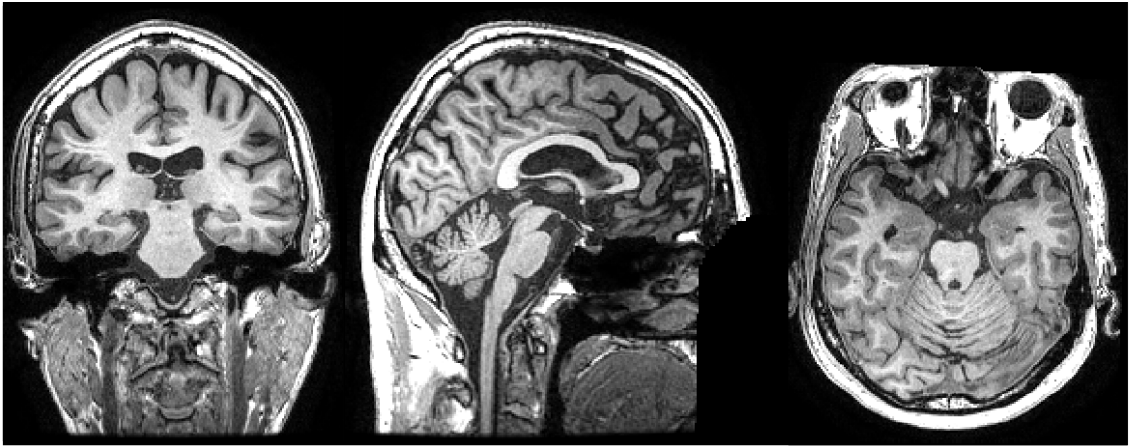
\includegraphics[scale=0.31]{acNormal.png}
    \centerline{Fonte: www.caddementia.grand-challenge.org}
    \label{fig:acNormal}
\end{figure}

\begin{figure}[h]
    \centering
    \caption{Imagem de uma pessoa diagnosticada com (AD)}
    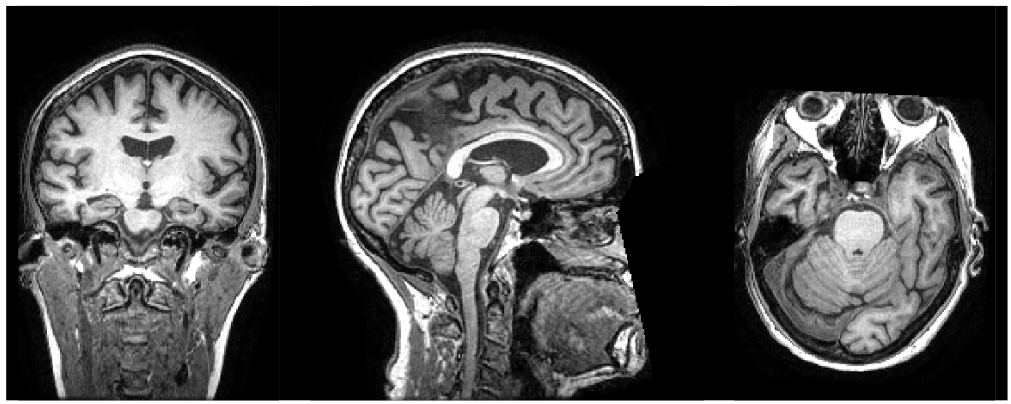
\includegraphics[scale=0.35]{adAlzhaimer.png}
    \centerline{Fonte: www.caddementia.grand-challenge.org}
    \label{fig:adAlzhaimer}
\end{figure}

Uma característica importante do sintoma da DA é perda dos neurônios da chamada massa cinzenta do cérebro, especialmente em regiões do córtex. Com isso é possivel verificar uma diminuição do volume dessa região. 
Na Figura \ref{fig:acNormal}  temos um exemplo de imagem de MRI de pessoa diagnosticada normal. Já na 
Figura \ref{fig:adAlzhaimer}  temos exemplo de uma pessoa diagnosticada com DA. Como já mencionado anteriormente temos alguns sistemas CAD, que com o auxílio de técnicas de processamento digital de imagens podem ajudar profissionais da saúde no diagnóstico.


\section{Aquisição de Imagens}

\subsection{Ressonância Magnética}
A imagem por ressonância magnética é hoje um método de diagnóstico já estabelecido na prática  pelas clínicas e em crescente desenvolvimento . Por razões físicas e pela abundância, o núcleo de hidrogênio (próton) é o elemento utilizado para produzir imagens de seres biológicos. Assim, para que esses átomos sejam orientados numa certa direção, é necessário um campo magnético intenso - habitualmente cerca de 1,5 Teslas. Entendida essa etapa, é possível associar o nome "magnética". Falta entender "ressonância" \cite{hage2009imagem}. A etapa seguinte é a excitação. Sabe-se que cada núcleo de
hidrogênio “vibra” numa determinada frequência proporcional
ao campo magnético em que está localizado. Assim, em 1,5 T, o hidrogênio tem frequência de 63,8 MHz. O aparelho emite então uma onda eletromagnética nessa mesma frequência. Existe uma transferência de energia da onda emitida pelo equipamento para os átomos de hidrogênio, fenômeno conhecido como ressonância \cite{hage2009imagem}. O aparelho utilizado na  ressonância magnética  pode ser visualizado na figura \ref{fig:ressonaciaAparelho}.

\begin{figure}[h]
    \centering
    \caption{Aparelho de Ressonância Magnética}
    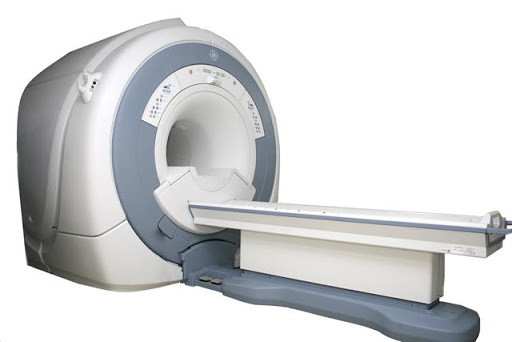
\includegraphics[scale=0.35]{figuras/ressonaciamagnetica.jpg}
    \centerline{Fonte: www.cediacimagem.com.br}
    \label{fig:ressonaciaAparelho}
\end{figure}


As imagens de RM têm maior capacidade de demonstrar diferentes estruturas no cérebro e têm facilidade em demonstrar mínimas alterações na maioria das doenças como por exemplo doença de Alzheimer. Na figura \ref{fig:ressonacia}, podemos ver exemplo da imagem gerada pela ressonância magnética (RM. A imagem por ressonância magnética é o método de diagnóstico por imagem não-invasivo mais sensível para avaliar partes moles, particularmente o encéfalo, porém trata-se de uma técnica onerosa. Ela apresenta grande potencial diagnóstico, poucos efeitos deletérios e muitos benefícios a serem obtidos com o seu uso \cite{mazzola2009ressonancia}. Com isso, o uso crescente dos computadores em aplicações clínicas e o desenvolvimento de novas ferramentas por dezenas de fabricantes geraram a necessidade de um método padrão para arquivamento e transferência dessas imagens e informações entre todos os dispositivos, independente do formato adotado pelo fabricante de origem, esse padrão e conhecido como DICOM \cite{grauer2009working}.


O DICOM é um conjunto de normas criado para garantir a troca e o armazenamento seguro das imagens radiológicas. A norma foi criada com o objetivo de facilitar a interpretação das informações provenientes da digitalização dos exames médicos \cite{graham2005dicom}. Com a chegada da informática e o uso de imagens digitais em clínicas e hospitais, fez com que se tornasse necessário ter uma padronização no formato das imagens geradas pelos equipamentos. O DICOM surgiu como uma solução para a uniformização dessa comunicação \cite{mustra2008overview}. Com a padronização, todos os tipos de exames – tomografias, ressonâncias, radiografias, são armazenados em um formato único, permitindo a troca entre equipamentos de marcas distintas. A criação desse conjunto de normas possibilita que as imagens sejam reconhecidas e visualizadas em qualquer um desses equipamentos \cite{graham2005dicom}. Esse conjunto de normas foi criado em 1983, no Colégio Americano de Radiologia, em parceria com a Associação Nacional Elétrica Americana \cite{varma2012managing}.

O DICOM também possibilita o acesso das informações em outros dispositivos. Os profissionais podem acessar as imagens e exames de pacientes em aparelhos móveis, como tablets e smartphones. Dessa forma, é possível fazer o acompanhamento e até diagnósticos prévios à distância \cite{noumeir2006benefits}. A padronização traz benefícios ainda para os exames enviados pela internet, pois as imagens não sofrem perda na qualidade, o que poderia prejudicar a interpretação feita pelos médicos. Garantir a padronização de imagens médicas já foi um desafio para as instituições de saúde \cite{noumeir2006benefits}. A variação em uma imagem, a falta de legibilidade ou de nitidez prejudicavam a avaliação dos exames e seus resultados. A criação do DICOM foi fundamental para garantir a segurança nos processos de análises radiológicas e clínicas \cite{liu2007medical}.



\begin{figure}[h]
    \centering
    \caption{Imagens de ressonância magnética}
    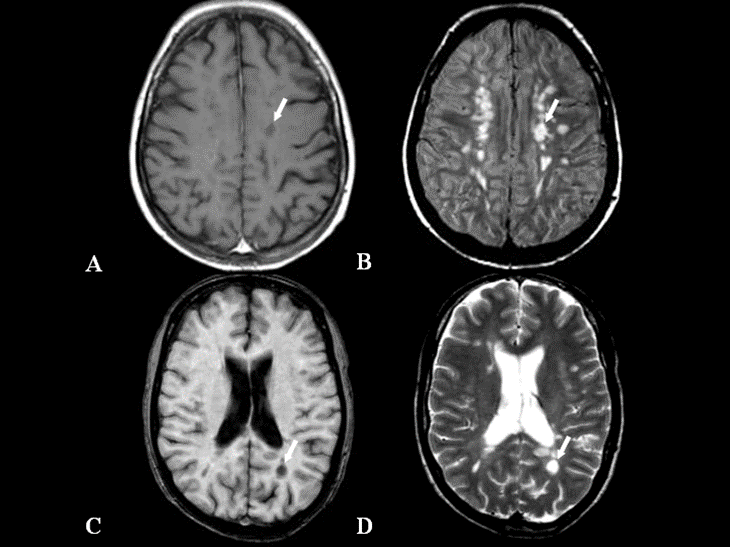
\includegraphics[scale=0.35]{figuras/image006.png}
    \centerline{Fonte: www.scielo.br}
    \label{fig:ressonacia}
\end{figure}

\subsection{Tomografia computadorizada}

A tomografia computadorizada é uma técnica, que se baseia em raios-X, foi utilizada para aplicações clínicas por volta da década de 70, uma vez que
torna possível examinar o encéfalo e, com maior clareza, os
limites do sistema ventricular e as partes ósseas do crânio. O
aparelho consiste em uma fonte de raios-X que é acionada ao
mesmo tempo em que realiza um movimento circular ao redor
da cabeça do paciente, emitindo um feixe de raios-X em forma
de leque. No lado oposto a essa fonte, está localizada uma série de detectores que transformam a radiação em um sinal elétrico que é convertido em imagem digital \cite{garib2007tomografia}.

O aparelho de tomografia computadorizada tradicional apresenta três componentes principais : 1) o gantry, no interior do qual se localizam o tubo de raios-x e um anel de detectores de radiação, constituído por cristais de cintilação; 2) a mesa, que acomoda o paciente deitado e que, durante o exame, movimenta-se em direção ao interior do gantry e 3) o computador, que reconstrói a imagem tomográfica a partir das informações adquiridas no gantry.

\begin{figure}[h]
    \centering
    \caption{Imagens de exemplo Tomografia computadorizada}
    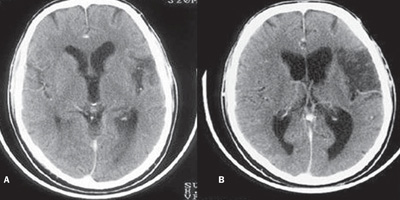
\includegraphics[scale=0.60]{figuras/tomografia-computadorizada-do-cranio-tesla-imagem.jpg}
    \centerline{Fonte:www.teslaimagem.com.br}
    \label{fig:tomocomp}
\end{figure}

Devemos ter conhecimento que a imagem de tomografia computadorizada ainda apresenta uma terceira dimensão, representada pela espessura do corte. Assim, uma outra palavra deve ser familiar aos profissionais que trabalham com imagens tridimensionais: o voxel. Denomina-se voxel a menor unidade da imagem na espessura do corte, podendo variar de 0,5 a 20mm, a depender da região do corpo a ser escaneada e da qualidade da imagem desejada. Na figura \ref{fig:tomocomp} podemos ver exemplo de imagem gerada apartir de uma  tomografia computadorizada, veja que  a imagem e muito semelhante a imagem de ressonância magnética.




\subsection{Pet Scan}
A tomografia por emissão de pósitrons (PET) associada à tomografia computadorizada (PET/CT), introduzida em 1998, teve impacto notório, principalmente na oncologia \cite{parks1988cerebral}. A sua grande vantagem é a propriedade de produzir imagens que identificam as alterações metabólicas e funcionais em todo o organismo completo e também é capaz de detectar os tumores até mesmo antes que se manifestem anatomicamente. O PET/CT é um dos exames de imagem mais modernos usados  por exemplo na oncologia. Ele combina duas modalidades de exame, a tomografia computadorizada, e a emissão de pósitrons, capaz de detectar a atividade metabólica das células do corpo \cite{parks1988cerebral}. Na figura \ref{fig:petct}, podemos ver um exemplo da imagem gerada pelo PET/CT.

\begin{figure}[h]
    \centering
    \caption{Imagens de exemplo PET/CT do Cérebro}
    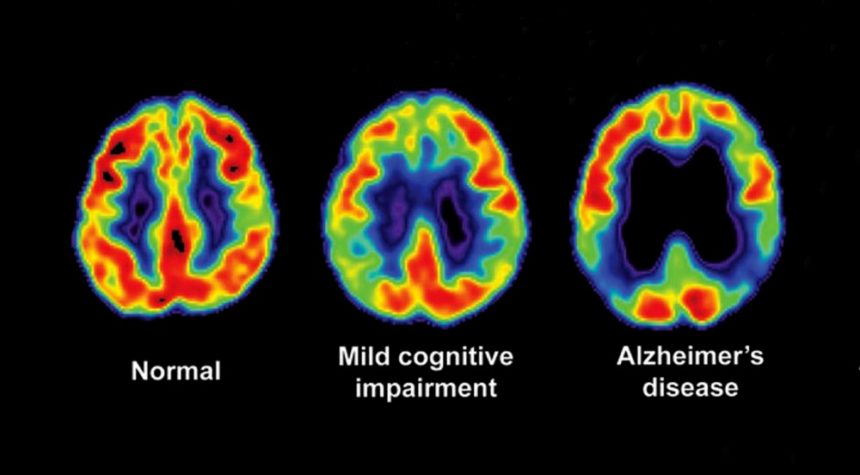
\includegraphics[scale=0.35]{figuras/alzheimersprogressionpet_1227001-860x475.jpg}
    \centerline{Fonte:www.dimen.com.br}
    \label{fig:petct}
\end{figure}

\begin{figure}[h]
    \centering
    \caption{Imagens de Exemplo Aparelho PET/CT}
    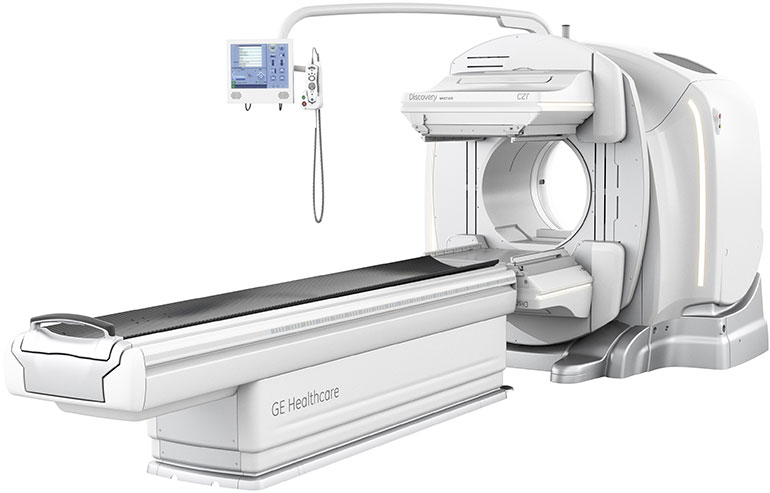
\includegraphics[scale=0.35]{figuras/discovery630-medicina-nuclear.jpg}
    \centerline{Fonte:www.cetac.com.br}
    \label{fig:petctapa}
\end{figure}

O PET-CT é indicado em casos suspeitos de câncer, para análise do estágio de um tumor, para avaliação de eficácia de tratamento, para planejamento de radioterapia, para verificar a saúde de corações que já tenham sofrido infartos e para analisar a função cerebral em detalhes.
Para realizá-lo, o paciente recebe, por via venosa, uma substância que emite baixas doses de radiação a base de glicose. Com isso, o médico consegue observar o consumo da glicose em cada parte do corpo e localizar possíveis problemas. Na figura
\ref{fig:petctapa} temos um exemplo do aparelho PET/CT, onde e realizado o exame.



\begin{table}[]
\caption{Comparativo das três formas de aquisição de imagem}
\label{fig:wrapfig}
\begin{tabular}{|l|l|l|l|}
\hline
 &
  \textbf{\begin{tabular}[c]{@{}l@{}}Ressonância \\ Magnética\end{tabular}} &
  \textbf{\begin{tabular}[c]{@{}l@{}}Tomografia \\ Computadorizada\end{tabular}} &
  \textbf{PET/Scan} \\ \hline
Técnica &
  \begin{tabular}[c]{@{}l@{}}As imagens são geradas em \\ alta definição através de \\ interação entre um \\ campo magnético,\\ ondas de rádio e o elemento\\ químico hidrogênio, \\ o mais abundante nos\\ tecidos corporais.\end{tabular} &
  \begin{tabular}[c]{@{}l@{}}A técnica da tomografia\\ utiliza raio-X em um \\ equipamento de \\ alta tecnologia,\\ que permite \\ fotografar o corpo \\ humano em \\ “fatias” e depois\\ reconstruir, \\ diferenciando os\\ tecidos através\\ da sua densidade.\end{tabular} &
  \begin{tabular}[c]{@{}l@{}}Tomografia \\ Por Emissão \\ de Pósitrons. \\ Utiliza radiação\end{tabular} \\ \hline
\begin{tabular}[c]{@{}l@{}}Tempo\\  de exame\end{tabular} &
  \begin{tabular}[c]{@{}l@{}}Mais demorado, com \\ duração de\\ cerca de 15-20 minutos \\ nos exames \\ mais simples até \\ cerca de 60-80\\ minutos nos de \\ maior complexidade.\end{tabular} &
  \begin{tabular}[c]{@{}l@{}}Muito rápido, com duração\\ média em torno de\\ 2-5 minutos.\end{tabular} &
  \begin{tabular}[c]{@{}l@{}}Após um repouso \\ de 60 minutos,\\ necessário para \\ a concentração \\ do radiofármaco\\ no organismo, \\ é feita a aquisição \\ das imagens\end{tabular} \\ \hline
Contraste &
  \begin{tabular}[c]{@{}l@{}}Utiliza a substância \\ gadolínio por\\ via endovenosa. \\ Reações alérgicas\\ são raríssimas. Pessoas com\\ insuficiência renal grave \\ não devem realizar o exame.\end{tabular} &
  \begin{tabular}[c]{@{}l@{}}Utiliza substância a\\  base de iodo, \\ que pode ser ingerida,\\  injetada por\\ via endovenosa ou\\  introduzida por \\ via retal ou\\ sondas/cateteres.\end{tabular} &
  \begin{tabular}[c]{@{}l@{}}Utiliza substância \\ chamada de \\ FDG\\ (fluordesoxiglicose).\\ Essa medicação\\  nada mais é do\\ que glicose (açúcar) \\ levemente \\ alterada \\ quimicamente com \\ uma partícula\\  radioativa (o flúor)\end{tabular} \\ \hline
Vantagens &
  \begin{tabular}[c]{@{}l@{}}Não utiliza radiação,\\  não há efeitos\\  colaterais ou danos à saúde \\ pela exposição ao campo \\ magnético e ondas de rádio \\ e menor chance de \\ reação alérgica. \\ Há maior diferenciação\\  na imagem \\ de tecidos moles e mais \\ técnicas que \\ permitem estudo \\ de doenças e tumores.\end{tabular} &
  \begin{tabular}[c]{@{}l@{}}É menos sensível à \\ movimentação \\ do paciente durante \\ a realização do exame, \\ não apresenta risco a \\ pacientes com \\ dispositivos médicos\\  implantáveis.\\ Também é um exame mais \\ rápido de ser realizado e o \\ aparelho é maior e\\  mais aberto. \\ Exame de menor custo.\end{tabular} &
  \begin{tabular}[c]{@{}l@{}}Permite o mapeamento \\ de diferentes \\ substâncias químicas \\ no organismo.\\ A vantagem da \\ PET Scan sobre os\\  demais exames de \\ imagens é que \\ ela permite\\  medir a atividade \\ metabólica das\\  lesões demonstrando \\ assim o grau de \\ atividade delas.\end{tabular} \\ \hline
\end{tabular}
\caption{Fonte: Publicação segundo www.ecomax-cdi.com.br}
\end{table}


Na tabela  \ref{fig:wrapfig}, pode observar uma comparação sobre alguns critérios de cada metódo de aquisição de imagens  mecionadas no texto. Naturalmente cada exame tem outras características não abordadas no texto. Depois de termos a imagem no padrão DICOM, podemos utiliza  técnicas de processamento de imagens por outro processo, como por exemplo a normalização da imagem.




\section{Processamento de Imagem}

Segundo Crosta (1999) o processamento de imagens é um método para converter uma imagem em forma digital e executar algumas operações nela, por exemplo
um método para converter uma imagem em forma digital, com o objetivo de obter versões aprimoradas da imagem aplicando filtros de sinais, como exemplo, ou extrair algumas informações relevantes. Esta área vem sendo objeto de crescente interesse por permitir a criação de grande número de aplicações que necessitem de extração de informação de imagens \cite{crosta1999processamento}.

O sistema visual humano tem uma grande capacidade de reconhecer padrões. No entanto, ele dificilmente é capaz de processar o enorme volume de dados presentes num estímulo visual. Por isso o principal objetivo do processamento de imagens é o de remover essas barreiras, inseparáveis ao sistema visual humano, facilitando a extração de informações a partir de imagens. Nesse contexto, o processamento digital deve ser encarado como uma fase preparatória, embora quase sempre obrigatória, da atividade de interpretação das representações gráficas \cite{crosta1999processamento}.

Uma das primeiras aplicações em processamento digital imagens foi no começo deste século,
onde buscavam-se formas de aprimorar a qualidade de impressão de imagens digitalizadas
transmitidas através do sistema Bartlane de transmissão de imagens por cabo submarino entre
Londres e Nova Iorque. Os primeiros sistemas Bartlane, no início da década de 20, codificavam
uma imagem em cinco níveis de intensidade distintos. Esta capacidade seria expandida, já em
1929, para 15 níveis, ao mesmo tempo em que era desenvolvido um método aprimorado de
revelação de filmes através de feixes de luz modulados por uma fita que continha informações
codificadas sobre a imagem. Mas o grande impulso para a área de Processamento de Imagens viria cerca de três
décadas mais tarde, com o advento dos primeiros computadores digitais de grande porte e o
início do programa espacial norte-americano \cite{gonzalez2010processamento}. O uso de técnicas computacionais de
aprimoramento de imagens teve início no Jet Propulsion Laboratory (Pasadena, California -
EUA) em 1964, quando imagens da lua transmitidas por uma sonda Ranger2
eram processadas por computador para corrigir vários tipos de distorção inerentes à câmera de TV acoplada à
sonda \cite{gonzalez2010processamento}. Estas técnicas serviram de base para métodos aprimorados de realce e restauração de
imagens de outros programas espaciais posteriores, como as expedições tripuladas da série
Apollo, por exemplo. De 1964 aos dias atuais, a área de processamento de imagens vem apresentando
crescimento expressivo e suas aplicações permeiam quase todos os ramos da atividade humana \cite{de2000processamento}.
Em Medicina, o uso de imagens no diagnóstico médico tornou-se rotineiro e os avanços em
processamento de imagens vêm permitindo tanto o desenvolvimento de novos equipamentos
quanto a maior facilidade de interpretação de imagens produzidas por equipamentos mais
antigos, como por exemplo o de raio X. Em Biologia, a capacidade de processar
automaticamente imagens obtidas de microscópios, por exemplo, contando o número de células
de um certo tipo presentes em uma imagem, facilita sobremaneira a execução de tarefas
laboratoriais com alto grau de precisão e repetibilidade. 






\section{Normalização MNI}

A normalização espacial é um processo de transformação de uma imagem MRI
para corresponder a um cérebro modelo padrão.
O \textit{Montreal Neurological Institute} (MNI) desenvolveu uma série de imagens semelhantes ao  modelo de coordenadas cerebrais Talairach que foram baseadas na média de muitas imagem de exames de ressonância magnética (MRI) normais. Essas imagens são normalmente utilizadas por \textit{software} de normalização espacial automatizada e devem refletir a média \cite{moraisinfluencia}. O \textit{International Consortium of Brain Mapping} (ICBM) adotou esses modelos como um padrão internacional. A normalização espacial remodela o cérebro de um indivíduo para corresponder à forma e ao tamanho de uma imagem padrão. Esta é uma etapa crucial necessária para análises estatísticas em nível de grupo. Os modelos padrão mais populares são derivados de exames de ressonância magnética de jovens e adultos. 

Na figura \ref{fig:normalizationmri} podemos ver as etapas do processamento da imagem. As imagens funcionais para cada modelo são realinhadas para corrigir o movimento do mesmo e, em seguida, são registradas em conjunto com uma imagem estrutural. Se necessário, as imagens são normalizadas espacialmente para alinhar os cérebros entre os modelos. A análise estatística tenta detectar áreas que tenham sido ativadas pela manipulação experimental. Os resultados podem ser exibidos em imagens estruturais individuais ou médias.

A análise estatística pode envolver qualquer um de diversos métodos , a maioria dos quais resulta em algum índice a cada \textit{voxel} de como o cérebro reagiu à manipulação de interesse experimental. Este mapa de ativação pode ser \textit{thresholded} para identificar regiões do cérebro ativadas. Se escaneamos vários modelos,então podemos realizar uma interpolação entre os modelos para
encontrar regiões resultantes do processo  \cite{brett2002problem}. A estimativa de localização de uma ativação estará sujeita a algum erro devido a ruído estatístico.

A etapa final da análise é a rotulagem de as áreas ativadas. As etiquetas podem estar em termos de coordenadas estereotáxicas, macroanatomia,microanatomia ou  em função.

\begin{figure}[h]
    \centering
    \caption{Estágios do processamento de imagem}
    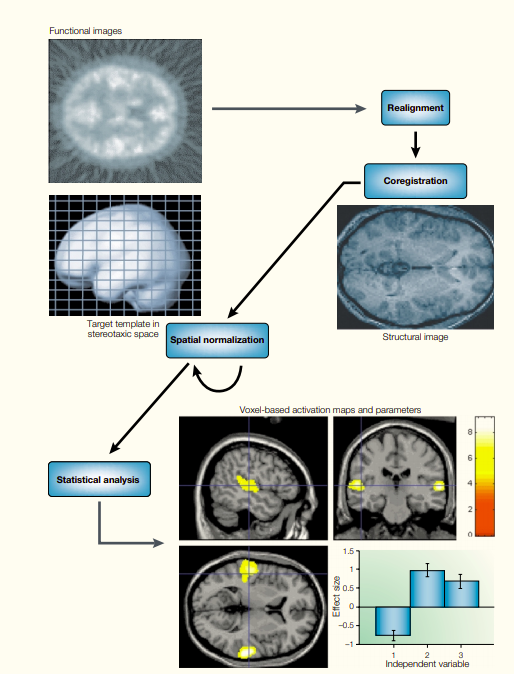
\includegraphics[scale=0.40]{normalization_mri.png}
    \centerline{Fonte: www.nature.cm}
    \label{fig:normalizationmri}
\end{figure}

A normalização está intimamente relacionada à ativação da rotulagem. Uma normalização bem sucedida requer uma forte concepção de como a anatomia do cérebro corresponde ao funcionamento, porque geralmente é
projetado para dar a melhor correspondência espacial de áreas homólogas entre indivíduos. A normalização também afeta a rotulagem que
é baseado em informações de um modelo cérebro; se a normalização não for bem sucedida no alinhamento das áreas funcionais correspondentes, então definições de áreas funcionais de outros indivíduos não serão aplicáveis. Para realizar esse processo de normalização funcional utilizamos algumas ferramentas de normalização avançada. 

\section{Ferramentas de normalização avançadas}

Existem  algumas ferramentas para trabalhar com processamento de imagem, sendo uma das mais  especificas quanto a ferramenta ANTs \footnote[1]{https://github.com/ANTsX/ANTs} ( \textit{Advanced Normalization Tools}). ANTs é um conjunto de ferramentas, que possui  diversas bibliotecas que nos permite explorar estatisticamente grandes conjuntos de imagens biomédicas.
ANTs depende da biblioteca \textit{Insight ToolKit} (ITK) , uma biblioteca de processamento de imagens médicas amplamente usada para a qual os desenvolvedores de ANTs contribuem para a biblioteca. O ITK é
patrocinado pelo NIH \cite{tustison2014advanced}. Fundada em 2008 com a conceituada estrutura de registro de imagens Symmetric Normalization, a biblioteca ANTs cresceu para incluir funcionalidades adicionais. Aprimoramentos recentes incluem recursos de estatística, visualização e aprendizado profundo por meio da interface com o projeto estatístico R (ANTsR) e o Python (ANTsPy). Adicionalmente, as extensões de aprendizado profundo correspondentes ANTsRNet e ANTsPyNet (construídas nas populares bibliotecas TensorFlow / Keras) contêm várias arquiteturas de rede populares e modelos treinados para aplicativos específicos \cite{tustison2014advanced}.

Existe também outra ferramenta de pre-processamento de imagem que é a  MINC Toolkit \footnote{https://bic-mni.github.io/}, que  também auxilia no processamento de imagem do formato DICOM (comunicação de imagens digitais em medicina). O formato de arquivo MINC  foi desenvolvido  e lançados por Peter Neelin em 1992 devido às suas frustrações em lidar com vários formatos de arquivo de diversos scanners e grupos de pesquisa. Nos anos seguintes, muitas ferramentas associadas (registro de imagem, normalização, visualização) foram escritas e também lançadas. O formato de arquivo MINC original e as ferramentas eram baseados no formato de dados NetCDF. A biblioteca e as ferramentas atuais do MINC são mantidas por um grupo de desenvolvedores em vários laboratórios de pesquisa de imagens em todo o mundo \cite{shafiei2020spatial}.

 
\section{Segmentação de Imagem}

A segmentação é o processo que subdivide uma
imagem em regiões que satisfaçam alguns critérios
de similaridade ou descontinuidade pré-definidos. Frequentemente, o resultado não é uma imagem, mas um conjunto de regiões/objetos.
A definição para a segmentação de imagens esta diretamente relacionada à área na qual
será aplicada. Dentro da área de visão computacional, a segmentação refere-se ao
processo de decomposição de uma imagem digital em vários segmentos (regiões) que a
formam (Jain, 1989). Já para a área de processamento digital de imagens de
sensoriamento remoto a segmentação de imagem é a parte da análise de imagem que
trata da definição de objetos geográficos ou regiões em uma imagem (Moik, 1980). Geralmente a segmentação é baseada em propriedades
dos níveis de cinza da imagem como descontinuidade e similaridade.

As descontinuidades encontradas em uma imagem podem ser pontuais, linhas ou os
limites (bordas) de um objeto. Essas feições, sobressaem numa imagem, seja por possuir
tons de cinza distintos a região na quais estão inseridas (caso de pontos e linhas) ou por
assinalarem mudanças bruscas de tons de cinza entre regiões (caso de bordas e linhas).
Os algoritmos desenvolvidos para detectar essas descontinuidades usualmente usam a
convolução, implicando no uso de máscaras.
Os métodos de detecção de descontinuidades, mais particularmente os de detecção de
linhas e de bordas, apresentam geralmente como resultados falhas de detecção. Portanto,
esses métodos devem ser seguidos de processamentos visando tratar essas falhas. As
técnicas de processamento que realizam esse tipo tratamento não serão abordadas aqui,
maiores detalhes a respeito ver  \cite{gonzalez2010processamento}. 

A detecção de similaridade tem como fundamento a observação do interior dos objetos e
não as fronteiras que os delimitam. Para tanto, parte da idealização que os pixels que
compõe um objeto têm propriedades similares enquanto que pixels de objetos distintos
têm propriedades distintas.
A formulação básica adotada para este tipo de abordagem é dada por \cite{fu1981survey}.
Segundo o autores, se considerarmos R como sendo uma imagem, a segmentação é a
decomposição de R em n regiões R1, R2, ..., Rn de tal forma que:



\begin{itemize}
  \item $ \cup_{\textit{i}=1}^n R_{i} = R   $
  \item $ R_{i}$ , é conectada, $i =1,2,...,n $
  \item $ R_{i} \cap{} R_{j} = \varnothing, \forall i \neq j $
  \item $ Pu(R_{i})= \textit{verdadeiro} \hspace{0.2cm} \forall \hspace{0.2cm} i $
  \item $ Pu(R_{i}  \cap{}  R_{j})= \textit{falso} \hspace{0.2cm} \forall \hspace{0.2cm} i  \neq j$
\end{itemize}


Pode existir um número de possíveis partições, mas a seleção de um conjunto adequado
de regiões depende da escolha da propriedade Pu associada à região, ou seja, do
predicado de uniformidade dos pixels da região \cite{pavlidis2013structural}. O conceito de segmentação da forma com que é apresentado idealiza o mundo real de
forma conveniente para diversas aplicações. Entretanto, cabe lembrar que é uma
invenção da mente humana e que embora seja uma boa abordagem para materializar
soluções para trabalhos de análise de imagens, pode em algumas situações levar a
resultados insatisfatórios \cite{davies2004machine}. 



\section{Aprendizado de Máquina}

Na computação, problemas são geralmente resolvidos por um algoritmo que especifica uma sequência de passos para a solução. Entretanto, é difícil definir um algoritmo que resolva alguns problemas que humanos realizam com facilidade diariamente, por exemplo, reconhecer um rosto ou compreender um texto \cite{watkins2001structural}. É difícil saber exatamente quais características do rosto devem ser observadas para que possamos reconhecê-lo mesmo quando aparece com um óculos, uma barba, ou de um ângulo totalmente diferente. Com imagens digitais, da mesma forma, não é fácil tornar explícito nosso o objeto que queremos rotular ou reconhecer na imagem \cite{watkins2001structural}.

Apesar da dificuldade de programar computadores para realizar essas tarefas complexas, elas hoje são frequente e constantemente realizadas usando a computação. Como por exemplo temos os carros autônomos, que utilizam algoritmos de aprendizado de máquina, para reconhecimento de objetos capturados pela câmera do veiculo. Outros casos
típicos que estão presentes no dia a dia da maioria das pessoas atualmente incluem sistemas de anti-spam como o do Gmail, que afirma ter precisão de 99,9\% para distinguir mensagens legítimas de spam e phishing, conforme Wen (2020), e o reconhecimento facial do Facebook, que usa fotos do usuário para criar um número único chamado gabarito e depois o compara a fotos, vídeos e lives para encontrar os outros conteúdos nos quais o usuário aparece, \cite{bachrach2012personality} .

Esses dois exemplos, assim como inúmeras outras soluções semelhantes, usam
técnicas de Inteligência Artificial (IA), especialmente o Aprendizado de Máquinas (\textit{Machine Learning}), para instruir computadores a realizar tarefas altamente complexas cuja solução dificilmente poderia ser codificada de maneira explícita através de um algoritmo e que também não poderiam ser realizadas com a mesma eficiência por
humanos, dada a imensa quantidade de informações que precisam ser consideradas para sua execução.

Um problema para o Aprendizado de Máquinas, segundo Mitchell (1997), pode
ser definido precisamente como melhorar alguma medida de desempenho P quando executando uma tarefa T através de algum tipo de experiência de treinamento E. Por exemplo, aprender a filtrar spam é aprender uma função (hipótese) que mapeia qualquer e-mail
de entrada para um rótulo de spam ou não-spam. Quando esses três componentes (T , P ,
E) estão especificados, tem-se um problema de aprendizado bem definido \cite{mitchellmachine}.

Tarefas de classificação têm como retorno um valor de um espaço discreto, comu-
mente chamado atributo-alvo ou classe-alvo. O tema da classificação é bastante estudado
por comunidades de áreas como banco de dados, mineração de dados e recuperação de
informações. A noção geral do problema de classificação, para Manning, Raghavan e
Schütze (2008), é a de que: dado um conjunto de classes deve-se determinar a qual delas
um determinado objeto pertence. Uma das técnica de Aprendizado de Máquina é a classificação utilizando redes neurais profundas. 

\section{Redes Neurais Profundas}

As redes neurais profundas conhecidas como \textit{Deep Neural Networks} são definas segundo Simon \cite{haykin2007redes} redes neurais são sistemas com nós interconectados que funcionam como os neurônios do cérebro humano. Usando algoritmos, elas podem reconhecer padrões escondidos e correlações em dados brutos, agrupálos e classificálos, e com o tempo aprender e melhorar continuamente.

O aprendizado profundo permite que modelos computacionais compostos de múltiplas camadas de processamento aprendam representações de dados com múltiplos níveis de abstração. Esses métodos melhoraram drasticamente o estado da arte em reconhecimento de fala, reconhecimento de objetos visuais, detecção de objetos e muitos outros domínios, como descoberta de drogas e genômica. O aprendizado profundo descobre uma estrutura complexa em grandes conjuntos de dados usando o algoritmo de retro propagação para indicar como uma máquina deve alterar seus parâmetros internos que são usados para calcular a representação em cada camada da representação na camada anterior. Redes profundamente convolucionais trouxeram avanços no processamento de imagens, vídeo, fala e áudio.


As redes neurais podem existir com apenas uma camada de neurônios, situação em que, apesar de trabalharmos com uma rede neural, não estamos utilizando \textit{deep learning}.
Um exemplo de rede neural rasa é aquele que possui apenas uma camada oculta. Isso significa que teremos apenas uma camada oculta de neurônios entre os dados de entrada e saída da rede.

Na prática, quando as redes neurais possuem mais de duas camadas ocultas, trata-se de \textit{deep learning}. Estas camadas ocultas também são compostas por neurônios, sendo que o valor de cada um será definido da mesma forma que nas redes neurais rasas. Na Figura \ref{fig:redesneuraisprof} temos exemplo de rede neural profunda. Um ponto importante a se observar nas redes neurais profundas é que o significado do resultado (valor) de cada neurônio existente nas camadas ocultas costuma ser obscuro, não sendo possível para nós a sua interpretação. Teremos apenas as evidências do resultado final da rede neural, que poderá melhorar ou não de acordo com a adição de mais camadas ocultas a rede \cite{goodfellow2016deep}. Também é importante ressaltar que para cada neurônio temos uma função de ativação.

\begin{figure}[h]
    \centering
    \caption{Redes neurais profundas}
    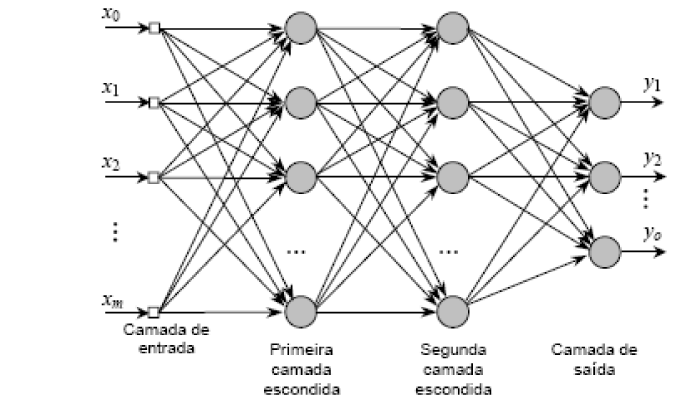
\includegraphics[scale=0.40]{redesneuraisprofundas.png}
    \centerline{Fonte: www.nature.cm}
    \label{fig:redesneuraisprof}
\end{figure}


As funções de ativação são um elemento extremamente importante das redes neurais profundas. Elas basicamente decidem se um neurônio deve ser ativado ou não. Ou seja, se a informação que o neurônio está recebendo é relevante para a informação fornecida ou deve ser ignorada \cite{goodfellow2016deep}. Podemos ver a fórmula abaixo, como a função de ativação é mais uma camada matemática no processamento da rede.

\[ Y = Ativacao(\sum (peso * entrada) + bias) \]

A função de ativação é a transformação não linear feita ao longo do sinal de entrada. Esta saída transformada é então enviada para a próxima camada de neurônios como entrada. Na função temos o peso que é atribuido a cada neurônio,eo valor de entrada é também temos o bias que é como o intercepto adicionado em uma equação linear. É um parâmetro adicional na rede que é usado para ajustar a saída junto da soma ponderada das entradas para o neurônio. Ou seja, bias é uma constante que ajuda o modelo de uma maneira que ele possa se adaptar melhor aos dados fornecidos. Outro pornto importante é os tipos de funções de ativação que são mais utilizadas nos modelos das redes, abaixo temos algumas delas.


ReLU é a função de ativação mais amplamente utilizada ao projetar redes neurais atualmente. Primeiramente, a função ReLU é não linear, o que significa que pode facilmente copiar os erros para trás e ter várias camadas de neurônios ativados pela função ReLU. A principal vantagem de usar a função ReLU sobre outras funções de ativação é que ela não ativa todos os neurônios ao mesmo tempo \cite{gomide2012redes}.



A função logística ou sigmoide produz valores no intervalo [0, 1].
 A maior vantagem sobre a função de etapa e a função linear é que não é linear. Esta é uma característica incrivelmente interessante da função sigmóide. Isto significa essencialmente que quando eu tenho vários neurônios com função sigmóide como função de ativação – a saída também não é linear. A função varia de 0 a 1 tendo um formato S  \cite{gomide2012redes}.


A função Softmax é uma generalização da função sigmoide para casos não-binários. Ela não costuma ser aplicada às camadas escondidas da rede neural, mas sim na camada de saída de problemas de classificação multiclasse, já que sua característica é produzir valores no intervalo [0, 1] onde sua soma é igual a 1. Ou seja, num problema com 3 classes, por exemplo, a função softmax vai produzir 3 valores, que somam 1, onde cada valor representa a probabilidade da instância pertencer a uma das 3 possíveis classes \cite{gomide2012redes}.

Existem diversos tipos de funções de ativação e esta é uma área de pesquisa ativa, à medida que a Inteligência Artificial evolui. Uma outra subárea das redes neurais, são redes  utilizadas para trabalhar com imagens digitais, essas redes são chamadas de redes neurais convolucionais.

\section{Redes Neurais Convolucionais}

Uma Rede Neural Convolucional (ConvNet / \textit{Convolutional Neural Network} / CNN) é um algoritmo de aprendizado profundo que receber como entrada uma imagem de entrada, atribuir importância (pesos e vieses que podem ser aprendidos) a vários aspectos / objetos da imagem e ser capaz de diferenciar um do outro  \cite{vargas2016estudo}. O pré-processamento exigido em uma ConvNet é muito menor em comparação com outros algoritmos de classificação. Enquanto nos métodos primitivos os filtros são feitos à mão, com treinamento suficiente, as ConvNets têm a capacidade de aprender esses filtros / características \cite{vargas2016estudo}.

Uma CNN é capaz de capturar com sucesso as dependências espaciais e temporais em uma imagem através da aplicação de filtros relevantes. A arquitetura executa um melhor ajuste ao conjunto de dados da imagem devido à redução no número de parâmetros envolvidos e à capacidade de reutilização dos pesos. Em outras palavras, a rede pode ser treinada para entender melhor a característica da imagem \cite{shalev2014understanding}. Na Figura \ref{fig:cnnref}, temos um exemplo de CNN e algumas das etapas da rede.



\begin{figure}[h]
    \centering
    \caption{Redes neural convolutional}
    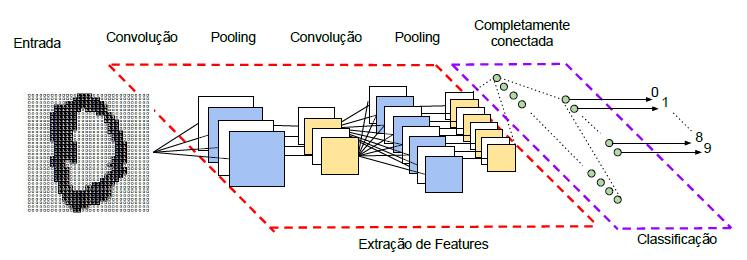
\includegraphics[scale=0.50]{cnn.jpg}
    \centerline{Fonte: www.nature.cm}
    \label{fig:cnnref}
\end{figure}

A convolução é uma operação linear que a partir de duas funções, gera uma terceira (normalmente chamada de feature map). No contexto de imagens, podemos entender esse processo como um filtro/kernel que transforma uma imagem de entrada.
Um kernel é uma matrix utilizada para uma operação de multiplicação de matrizes. Esta operação é aplicada diversas vezes em diferentes regiões da imagem. Normalmente o stride possui o valor 1, o que significa que a transformação será aplicada em todos os pixels da imagem \cite{shalev2014understanding}. Geralmente as CNN tem algumas configuraçoes que são comumente aplicadas como por exemplo o \textit{Padding}.

O \textit{Padding} é um processo em que alguns pixels são adicionados ao redor da imagem antes da operação de convolução, de forma a manter a dimensionalidade na imagem resultante durante a operação.


O \textit{Pooling} é um processo de \textit{downsamping}. É um processo simples de redução da dimensionalidade/features maps. Em uma forma leviana de pensar, podemos entender essa transformação como uma redução do tamanho da imagem.


A camada de  \textit{flatten} normalmente é utilizada na divisão das 2 partes da CNN (extração de características / rede neural tradicional). Ela basicamente opera uma transformação na matrix da imagem, alterando seu formato para um array. Por exemplo, uma imagem em grayscale de 28x28 será transformada para um array de 784 posições. A imagem abaixo ilustra essa operação.

E comun termos na rede uma camada de \textit{Dropout} que é utilizada para evitar que determinadas partes da rede neural tenham muita responsabilidade e consequentemente, possam ficar muito sensíveis a pequenas alterações. Essa camada recebe um hyper-parâmetro que define uma probabilidade de “desligar” determinada área da rede neural durante o processo de treinamento. Ao final da rede é colocada uma camada \textit{Fully connected}, onde sua entrada é a saída da camada anterior e sua saída são N neurônios, com N sendo a quantidade de classes do seu modelo para finalizar a classificação.

Dentro do modelo também temos outros parametros que configuramos, de acordo com volume de dados. Um desses parametros é o \textit{batch size} é um hiperparâmetro que define o número de amostras a serem trabalhadas antes de atualizar os parâmetros do modelo interno. Pense em um \textit{batch size} (lote) como um \textit{loop for} que iterando sobre uma ou mais amostras e fazendo previsões. No final do lote, as previsões são comparadas às variáveis de saída esperadas e um erro é calculado. A partir desse erro, o algoritmo de atualização é usado para melhorar o modelo, por exemplo, mover para baixo ao longo do gradiente de erro. Outro parametro importante  é o numero de \textit{epochs} (épocas) para treinamento do modelo. O número de épocas é um hiperparâmetro que define o número de vezes que o algoritmo de aprendizado funcionará em todo o conjunto de dados de treinamento. Uma época significa que cada amostra no conjunto de dados de treinamento teve a oportunidade de atualizar os parâmetros do modelo interno. Uma época é composta por um ou mais lotes \cite{hentschel2016fine}.

Portanto depois de configuramos o modelo, temos que ter uma forma de validar
o modelo da rede, para isso temos alguns formas de validação de modelos. Na proxima seção vamos apresentar formas de avaliação de modelos.

\section{Avaliação de Modelos de Aprendizado de Máquina}

Uma questão a se levar em conta na construção de Modelos de Aprendizado de
Máquina é que é preciso testá-los com os dados do caso concreto em que o modelo será
aplicado. Segundo Faceli (2011), de maneira geral, pode-se afirmar que não é possível estabelecer a priori que uma técnica de ML em particular se sairá melhor que qualquer outra
na resolução de um certo tipo de problema. É preciso, portanto, comparar os diferentes
modelos para escolher o mais adequado ao problema em questão.

Pode-se comparar modelos sob vários aspectos, por exemplo, explicabilidade,
tempo de aprendizado ou desempenho preditivo. Esse último aspecto costuma ser um
dos mais importantes na seleção do modelo e, no caso de problemas de classificação, é
avaliado através de métricas de erro computadas pelo resultado do classificador ao rotular
exemplos não apresentados ele em tempo de treinamento


\subsection{Matriz de Confusão}

Uma maneira de visualizar as medidas de desempenho de um classificador é por
meio de uma matriz de confusão. Nessa matriz uma das dimensões representa a classe ver-
dadeira (já conhecida) e a outra a classe predita pelo classificador. Normalmente coloca-se
nas linhas a classe verdadeira e nas colunas a classe predita. Nesse caso, em uma matriz
M cada um de seus elementos m ij apresenta o número de exemplos da classe i classifica-
dos como pertencentes à classe j.

Em problemas de duas classes, uma delas é dita classe Positiva e a outra classe
Negativa. Da observação da matriz de confusão pode-se extrair diferentes medidas referentes a cada classe, bem como algumas métricas compostas. A lista abaixo apresenta
algumas dessas medidas.


\begin{itemize}
 \item\textbf{Precisão}: Proporção  de exemplos positivos classificados corretamente entre todos aqueles preditos como positivos.
 
 
 \item\textbf{Sensibilidade ou revocação}: Corresponde à taxa de acerto na classe positiva. Também é chamada de Taxa de Verdadeiros Positivos (TVP).
 
 
 \item\textbf{Especificidade}: Corresponde à taxa de acerto na classe negativa. Seu complemento corresponde à Taxa de Falsos Positivos.
 
 
 
 \item\textbf{Precisão}: 
 Proporção de exemplos positivos classificados corretamente entre todos aqueles
preditos como positivos.
 
 \item\textbf{Taxa de erro na classe negativa}: 
  Corresponde à proporção de exemplos da classe negativa incorretamente classificados. Também conhecida como Taxa de Falsos Positivos (TFP).


  
 \item\textbf{Valor preditivo negativo}: 
  É uma espécie de precisão na classe negativa, isto é, corresponde à proporção de exemplos negativos classificados corretamente, entre todos os preditos como negativos.
 
 \item\textbf{Acurácia} :  Soma dos valores da diagonal principal da matriz pela soma de todos os elementos da matriz.
  
 \item\textbf{Taxa de Descobertas Falsas } : 
   É o complemento da Precisão. Dito de outra forma: dentre todos os exemplos classificados como positivos, quantos eram Falsos Positivos.
\end{itemize}


A Taxa de erro na classe negativa, também conhecida como Taxa de Falsos Po-
sitivos (TFP), e a Taxa de acerto na classe positiva, também conhecida como Taxa de
Verdadeiros Positivos (TVP), são particularmente importantes para a criação de Curvas
ROC, discutidas a seguir.

\subsection{Curvas ROC}

As métricas TVP e TFP, discutidas previamente, podem ser alisadas conjuntamente em um gráfico chamado Receiving Operating Characteristics (ROC), cujos princípios são discutidos em Metz (1978). Trata-se de um gráfico bidimensional plotado em
um espaço denominado “Espaço ROC”, onde o eixo X representa a Taxa de Falsos Po-
sitivos e o eixo Y a Taxa de Verdadeiros Positivos. Consideradas essas duas medidas, o
desempenho de um classificador pode ser plotado como um ponto nesse espaço.

Embora seja possível comparar dois classificadores simplesmente por seus pontos
no espaço ROC, a maneira mais usual é gerar uma Curva ROC. Para plotar uma dessas curvas é preciso que o algoritmo possa apresentar como resultado da classificação
uma probabilidade de o exemplo pertencer a classe positiva. Tendo como saída do algoritmo esse valor contínuo, pode-se estabelecer diferentes limiares acima dos quais o
exemplo seria classificado como positivo. Escolhendo-se diferentes limiares tem-se diferentes valores de TVP e TFP, permitindo que múltiplos pontos sejam representados no espaço ROC, um para cada limiar. Ao se unir esses pontos têm-se uma Curva ROC para
o classificador.

\begin{figure}[h]
    \centering
    \caption{Exemplo de Curvas ROC}
    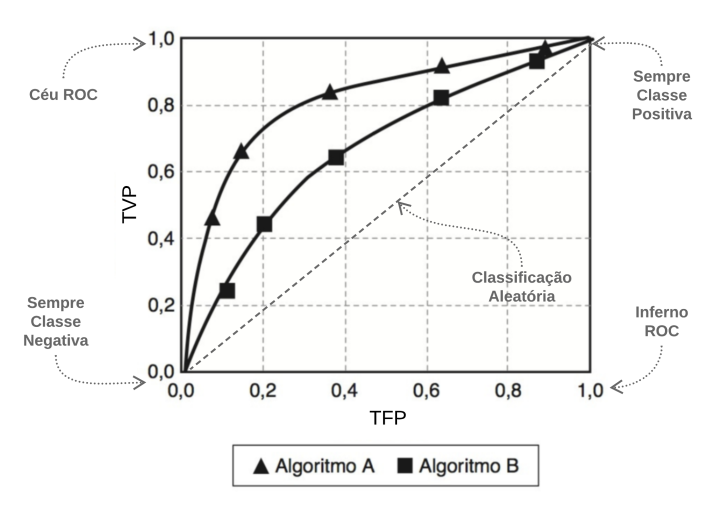
\includegraphics[scale=0.40]{curvarocexemplo.png}
    \centerline{Fonte: Adaptado de Faceli (2011)}
    \label{fig:curvarocexempl}
\end{figure}


A Figura \ref{fig:curvarocexempl}, ilustra um exemplo de comparação entre dois algoritmos através de
suas Curvas ROC. Na figura também estão representados os principais aspectos do espaço
ROC. A linha diagonal representa uma classificação aleatória. O ponto (0,1), chamado
de Céu ROC, representa classificações perfeitas, isto é, todos objetos da classe positiva
foram corretamente classificados como tal, assim como todos os objetos da classe negativa
foram corretamente classificados (não houve Falsos Positivos). O Ponto (1,0), dito Inferno
ROC, representa um classificador que erra todas as predições e os pontos (0,0) e (1,1)
representam classificadores que aplicam sempre a mesma classe para qualquer exemplo.




Além da avaliação visual obtida na observação das Curvas ROC, uma medida
objetiva usada para comparar os classificadores é a “Área Abaixo da Curva” ROC ou AUC (do inglês Area Under ROC Curve). A medida da AUC é um valor entre 0 e 1, sendo 1 o valor ideal. Assim, conforme explica Faceli (2011), ao comparar a AUC de dois
classificadores, aquele com maior AUC é considerado superior em termos de desempenho preditivo.


\section{Resumo do Capítulo}

Nesse capítulo foi apresentado os conceitos necessários para o desenvolvimento do trabalho. Apresentamos o Doença de Alzheimer, e quais são suas caracteristicas. Também foi mostrado forma de Aquisição de Imagens para o diagnóstico da doença. Foi abordado o conceito de Processamento de Imagens e algumas das técnicas como Normalização MNI e Segmentação.

Identificou-se o Aprendizado de Máquina como a capacidade de um algoritmo
de melhorar o desempenho na realização de alguma tarefa por meio da experiência e
mostrou-se que o treinamento supervisionado é uma das maneiras de atingir esse objetivo.
Foi apresentada o noção geral do problema de classificação como sendo a capacidade de
determinar a qual classe um determinado objeto pertence, dado um certo conjunto de
classes, e descreveu-se a classificação de imagens como um tipo particular deste problema.
A intersecção destes temas, isto é, a Classificação de Imagens MRI usando o Aprendizado de
Máquina Supervisionado mais precisamente as redes neurais convolucionais que foi sumarizada através da Figura \ref{fig:cnnref} .


\chapter{TRABALHOS RELACIONADOS}

Neste Capítulo são descritos trabalhos correlatos os quais realizaram pesquisas análogas
aos objetivos do presente trabalho. Os trabalhos nesta área têm recorrentemente considerado apenas um pequeno número de assuntos e
imagens, geralmente com dados selecionados (ou seja, revisados, preparados e organizados por especialistas), tais
como os Conjuntos de Dados Padronizados de MRI da ADNI. Além disso, com a falta de um protocolo padrão de avaliação, cada estudo empregou seus próprios critérios, com seus próprios dados divididos aleatóriamente. Isto não só dificulta a comparação entre os diferentes métodos, mas também geralmente
superestimam seu desempenho em um cenário do mundo real, onde os dados não serão prontamente
pré-processado, e muito provavelmente virá de diferentes fontes. 
Assim, são apresentados trabalhos resultantes de pesquisas sobre  processamento e classificação de imagens 3D e 2D utilizando  redes neurais convulucionais.

Em Kanghan Oh o autor apresenta uma abordagem usando o modelo CNN para quatro tarefas de classificação binária diferentes com base em imagens de ressonância magnética (MRI). Os autores dividiram o trabalho em duas tarefas, usando autoencoder convolucional (CAE) baseado em aprendizagem não supervisionada para a tarefa de classificação AD (\textit{alzheimer diagnosis}) vs NC (\textit{cognitively normal}) e aprendizagem de transferência supervisionada para resolver a tarefa de classificação pMCI vs. sMCI. Para detectar biomarcadores essenciais relacionados a AD e pMCI, os autores usaram um método de visualização baseado em gradiente que identificou os lobos temporais e parietais como regiões-chave para classificação.Os dados do experimento foram obtidos no ADNI, sendo total de  694 imagens de MRI. Com a idade dos pacientes entre 55 a 90 anos de idade. O modelo proposto obteve uma acurácia de 73,2\% \cite{oh2019classification}.



Ehsan Hosseini-Asl et al. propôs uma rede neural convolucional 3D profunda (3D-CNN) para classificar imagem de pessoas com AD. Os autores treinaram um autoencoder convolucional para capturar variações da forma anatômica em exames de ressonância magnética do cérebro. Após a extração dos recursos usando AE, eles realizam a classificação específica da tarefa com um 3D-CNN adaptável ao domínio de destino usando esses recursos. Os experimentos da CNN adaptável 3D (3D-ACNN) para o diagnóstico da doença de Alzheimer no conjunto de dados CADDementia MRI sem resultados de pré-processamento de remoção do crânio superam as precisões de vários classificadores comparadas em seu artigo.
Uma das abordagem dos autores foi se concentrara na adaptação de domínio  \textit{ domain adaptation}, ou adaptação
fonte-alvo, isso ocorre quando um classificador após o treinamento dos dados de origem são adaptados 
aos dados de destino.
Ao contrário do aprendizado supervisionado usual com um classificador treinado desde o início
minimizando uma perda quantitativa total de erros no
dados de treinamento, a adaptação do domínio minimiza a mesma perda
sobre o domínio de destino, atualizando o classificador, que tem
foram treinados no domínio de origem. Aproveitamos o aprendizado de recurso 
não supervisionado para transferir recursos encontrados na fonte
domínio para o domínio de destino, a fim de impulsionar a previsão
desempenho dos modelos CNN com camadas profundas \cite{hosseini2016alzheimer}. O programa do autor do 3D-CNN generaliza os recursos aprendidos e adaptados para outros domínios de teste no conjunto de dados ADNI \cite{hosseini2016alzheimer}.



Bae et.al desenvolveram um algoritmo baseado em CNN que usa varreduras de ressonância magnética para classificar pacientes com AD e controles CN. Os autores consideram cortes coronais de ressonância magnética cobrindo o lobo temporal medial para treinar e validar o algoritmo em diferentes etnias e níveis de educação. O conjunto de dados usado neste artigo foi um do ADNI e outro do SNUBH. Os resultados mostram áreas médias sob as curvas de 0,88-0,89 para validação de conjunto de dados, capaz de manter a alta precisão independentemente das características étnicas ou demográficas dos pacientes \cite{bae2020identification}. O algoritmo de  \cite{bae2020identification} considera a escala de atrofia do lobo 
temporal medial (MTA), que segundo os autores é amplamente utilizada na 
prática clínica para determinar a presença de neurodegeneração 
relacionada à DA. Esta escala também é usada como evidência neurodegenerativa para AD de acordo com as diretrizes/estrutura de pesquisa do National 
Institute on Aging and Alzheimer's Association 18 . 
Embora outras regiões também possam fornecer informações 
úteis para a classificação da DA, sabe-se que há uma ligeira
variabilidade interindividual nos padrões exatos de atrofia 19e 
a atrofia focada no 
lobo temporal medial (MTL) é o tipo mais comum \cite{bae2020identification}.


Sarraf e Tofighi propôs uma arquitetura de aprendizagem (LeNet) que foi treinada e testada com imagens AD e NC. Os autores realizaram o pré-processamento dos dados e, em seguida, o treinamento dos dados. Eles usam o conjunto de dados ADNI.Os dados utilizados estão no modelo 2D. 
Para o estudo, foram selecionados 30 pacientes com doença de Alzheimer (DA) e
idosos normais (24 mulheres e 19 homens)  com
uma idade média de 74,9 a 5,7 anos,  foram selecionados a partir da base de dados do ADNI.
A arquitetura do modelo realizado pelo autores foi LeNet-5. A Rede LeNet-5 implementada para  os dados fMRI  foram imagens 2D em JPEG usando o pacote de Neuroimaging Nibabel (http://nipy.org/nibabel/) e Python OpenCV
(opencv.org). Em seguida os autores, realizaram rotulagem  das imagens  para classificação binária de dados de Alzheimer vs. Normal. As imagens rotuladas foram convertidas em bancos de dados de armazenamento lmdb para alto rendimento a serem alimentados na plataforma Deep Learning.
Os dados foram divididos em três partes: treinamento
(60\%), validação (20\%) e teste (20\%). O número de
épocas foi definido como 30 e o tamanho do \textit{batch\_size }/ lote foi 64. O modelo testado  teve resultado de precisão de 96,4\%, para esse trablalho os autores não utilizaram o valor de AUC \cite{sarraf2016classification}.

 
\cite{rieke2018visualizing}  os autores utilizaram base de dados do ADNI. Para o estudo, os autores usaram os dados estruturais de ressonância magnética de pacientes com Alzheimer doença (AD) e controles normais (NC) da fase 1 do ADNI que foram incluídos
na "Coleção de ressonância magnética - Lista 1.5T padronizada - Anual 2 anos". Para cada
sujeito, esta coleta de dados oferece varreduras estruturais de ressonância magnética de todo o cérebro para até a três pontos de tempo (triagem, 12 e 24 meses; às vezes, várias varreduras
por visita). Excluímos exames com transtorno cognitivo leve (MCI) e dois exames
para o qual nosso pipeline de pré-processamento falhou. No total, nosso conjunto de dados compreende 969
varreduras individuais (475 AD, 494 NC) de 344 indivíduos (193 AD, 151 NC).
  
O  modelo proposto dos autores consiste em quatro camadas convolucionais (com tamanho de filtro 3 × 3 × 3 e
8/16/32/64 mapas de recursos) e duas camadas totalmente conectadas (128/64 neurônios; isso
a arquitetura é inspirada em um modelo em Khvostikov et al). No modelo nós aplicaram um \textit{batch normalization}  e \textit{pooling} após cada convolução e \textit{dropout} de 0,8 antes do
primeira camada totalmente conectada. A rede tem dois neurônios de saída com softmax
ativação. Treinamos com perda de entropia cruzada e o otimizador Adam (aprendendo
taxa 0,0001, tamanho de \textit{batch\_size }/ lote 5) por 20 épocas. Antes de alimentar o cérebro, as varreduras
rede, removemos o crânio e normalizamos cada voxel para ter média 0 e
desvio padrão 1 em todo o conjunto de treinamento. Os autores obtiveram um valor de acuracia de
0.78 ± 0.06 e um valor de  0.77 de AUC \cite{rieke2018visualizing}. 

 Neste artigo os autores \cite{feng2019deep}, propõem um novo framework composto por 3D-CNN. Os autores o chamaram de
FSBi-LSTM, o metodo proposto  é utilizado para o diagnóstico de DA. Especificamente,
proporam uma nova estrutura de rede LSTM em vez de
a camada FC em 3D-CNN. O método pode preservar o espaço
informações do mapa de recursos, tanto quanto possível. Comparado
com SBi-LSTM tradicional, extratos FSBi-LSTM comuns
informações da estrutura do cérebro intimamente conectadas de todas as
camadas SBi-LSTM, que podem representar informações de ‘‘ traço ’’ constantes
mação de cada assunto por meio da camada FC, em vez da parte
da informação da estrutura do cérebro. Realizamos extensa
experimentos baseados no conjunto de dados ADNI e demonstram o
eficácia do nosso método. Esse método também supera o
outros métodos competitivos usando CNN para identificação de rótulo
cátion. Além disso, melhoramos a explicação clínica de
aprendizado aprofundado em diagnóstico clínico por meio de blindagem cerebral
experimentos.













Na Tabela \ref{tab:comapreworker}, podemos ver uma pequena comparação dos métodos apresentados anteriormente. A tabela leva apenas a ACC, como comparativo dos métodos, por acreditarmos que como obtivemos propostas com diferentes dados e modelo de classificação podemos ter uma noção das pesquisas
relacionadas  sobre o assunto. Em seguida temos a Tabela \ref{tab:comparearq}, onde é descrito a arquitetura ea técnicas dos metodos pesquisados.


\begin{table}[h]
\centering
\caption{Comparação Entre Métodos Pesquisados  (ACC,\%)}
\label{tab:comapreworker}
\begin{tabular}{|l|l|l|l|}
\hline
\hspace{1cm} \textbf{Método}               & \textbf{Acurácia} & \textbf{Formato do Modelo} & \textit{\textbf{Dataset}}  \\ \hline

Kanghan Oh               &      73\%             &  \hspace{2cm}  3D    &    ADNI                       \\ \hline
Ehsan Hosseini-Asl et al &    91\%                 &  \hspace{2cm}  3D   &  ADNI, CADDementia                           \\ \hline
BAE et al.               &   89\%                 & \hspace{2cm}  2D    &   ADNI, SNUBH                          \\ \hline
Sarraf e Tofighi         &    96\%               &    \hspace{2cm}  2D   &    ADNI                       \\ \hline
RIEKE et al              &      78\%             &  \hspace{2cm}   3D &  ADNI
  \\ \hline
FENG et al             &      95\%             &  \hspace{2cm}   3D   &  ADNI

\\ \hline
\end{tabular}
\end{table}




\begin{table}[h]
\caption{Comparação Entre Métodos Pesquisados Técnicas dos Modelos}
\begin{tabular}{|l|l|}
\hline
\textbf{Método}          & \textbf{Técnica/Arquitetura}                                                                                        \\ \hline
Kanghan Oh               & \begin{tabular}[c]{@{}l@{}}Aprendizagem não supervisionada baseada \\ em autoencoder  convolucional.\end{tabular}                                                                                                                   \\ \hline
Ehsan Hosseini-Asl et al &                                                                                                                     \\ \hline
BAE et al.               &  \begin{tabular}[c]{@{}l@{}}   CNN 2D. Arquitetura \texit{inception v4}, baseada na GoogLeNet.\\ Utilizaram "Slices coronais"  de imagens 3D. \end{tabular}                                                                                                              \\ \hline
Sarraf e Tofigh          & \begin{tabular}[c]{@{}l@{}}CNN 2D. Arquitetura LeNet-5, adaptada.\\  Utilizaram "Slices" de imagens 3D.\end{tabular} \\ \hline
RIEKE et al &
  \begin{tabular}[c]{@{}l@{}}O modelo consiste em quatro camadas convolucionais\\  (com tamanho de filtro 3 × 3 × 3 e\\ 8/16/32/64 mapas de recursos) e duas camadas \\ totalmente conectadas (128/64 neurônios; isso\\ a arquitetura é inspirada em um modelo em Khvostikov et al.\end{tabular} \\ \hline
FENG et al               & CNN 3D. Arquitetura própria proposta, FSBI LSTM.                                                                    \\ \hline
\end{tabular}
\end{table}

\chapter{ABORDAGEM PROPOSTA}

O objetivo geral deste projeto é desenvolver, testar e avaliar uma ferramenta de Classificação de imagens de ressonância magnética (MRI), onde foi escolhido MRI, por ter uma melhor definição e qualidade na imagem, para mais detalhes ver Seção 2.3
, que possa auxiliar na detecção da doença de Alzheimer utilizando  \textit{deep learning}. Logo,
este Capítulo encontra-se organizado da seguinte forma: a Seção 4.1 expõe a metodologia utilizada como base para condução dos estudos realizados; a Seção 4.2 apresenta a  origem dos dados utilizados
a qual se baseia o desenvolvimento deste trabalho; a Seção 4.3 descreve como
foi realizado pre-processamento dos dados que foram utilizados no desenvolvimento do trabalho; Na
Seção 4.4 descreve a arquitetura do modelos desenvolvido juntamente com as tecnologias e conceitos de \textit{deep learning}; Por fim na
Seção 4.5  Descrevemos o resutados juntamnte com testes e métricas que foram utilizadas com os dados proposto no trabalho.


\section{Metodologia}
Neste capítulo, fornecemos detalhes da nossa implementação da proposta, incluindo o pré-processamento de imagens MRI no formato 3D,
a arquitetura da rede CNN, técnicas e ferramentas de otimização. Em particular, é importante destacar a
razão pela qual não utilizamos imagens em seu espaço original, e a necessidade de utilizar um padrão no formato dos dados.
Mesmo que as camadas convolutivas possam operar sobre dados com dimensões variáveis.
A otimização de um sistema de aprendizagem baseado em  \textit{deep learning} utilizando imagens sem nenhum padrão exige que ele aprenda
padrões discriminatórios invariantes a uma série de transformações, tais como a translação,
escala e rotação. Isto exigiria ter modelos com mais camadas, com tempos de treinamento crescentes,
e um número ainda maior de amostras, com todas as variações esperadas. Ao registrar nossas
imagens a um modelo padrão, podemos esperar que estruturas similares estejam aproximadamente no
mesma localização espacial, portanto podemos lidar com toda a imagem de uma só vez e automaticamente
determinar as regiões de interesse mais importantes.


Dentro do desenvolvimento da pesquisa realizada, foi analisado alguns conjuntos de dados para realizaçao da proposta. Um dos \textit{dataset}, pesquisado foi o oasis-brains \footnote{www.oasis-brains.org}, onde esse \textit{dataset} possui um conjunto de imagens tanto de MRI quanto de PET. Também foi analisado o dataset do desafio Caddementia \footnote{www.caddementia.grand-challenge.org}, onde eles disponibilizam \textit{dataset} que vieram  de três universidades 	
Erasmus MC, Medical Center e University of Porto. No entanto o conjunto dos dados disponíveis pelo desafio não  contem muitas MRI, todo dataset possui 509 imagens dividias em AD, NC, e MCI. Por fim  escolhemos utilizar na pesquisa o \textit{dataset} disponibilizado por ADNI, onde temos uma quantidade maior no conjunto dos dados e uma variedade  maior também com pessoas de faixa etarias distintas.   



\section{Dados}

Os dados utilizados na preparação desta proposta foram obtidos da Iniciativa de Neuroimagem da Doença de Alzheimer (ADNI) \footnote{https://adni.loni.usc.edu}. A base de dados da ADNI
foi lançado em 2003 pelo National Institute on Aging (NIA), o Instituto Nacional para o Envelhecimento
de Imagens Biomédicas e Bioengenharia (NIBIB), a Food and Drug Administration
(FDA), empresas farmacêuticas privadas e organizações sem fins lucrativos, como um fundo de 60 milhões de dólares,
Parceria público-privada de 5 anos. O principal objetivo da ADNI tem sido testar se
RM em série, PET, outros marcadores biológicos e avaliação clínica e neuropsicológica
pode ser combinado para medir a progressão da MCI e do início do AD. Determinação de
marcadores sensíveis e específicos de progressão muito precoce da AD destina-se a ajudar os pesquisadores
e clínicos para desenvolver novos tratamentos e monitorar sua eficácia, bem como diminuir
o tempo e o custo dos ensaios clínicos.

O principal investigador desta iniciativa é Michael W. Weiner, MD, VA Medical
Centro e Universidade da Califórnia - São Francisco. O ADNI é o resultado dos esforços de muitos
co-investigadores de uma ampla gama de instituições acadêmicas e corporações privadas,
e os sujeitos foram recrutados em mais de 50 locais nos Estados Unidos e Canadá. O objetivo inicial do ADNI era recrutar 800 sujeitos, mas o ADNI foi seguido pelo ADNIGO e ADNI-2.
 Até hoje, estes três protocolos já recrutaram mais de 1500 adultos, com 55 anos de idade
a 90, para participar da pesquisa, que consiste em indivíduos mais velhos cognitivamente normais,
pessoas com MCI cedo ou tarde, e pessoas com AD cedo. A duração do acompanhamento de
cada grupo é especificado nos protocolos para ADNI-1, ADNI-2 e ADNI-GO. Temas
originalmente recrutado para ADNI-1 e ADNI-GO tinha a opção de ser seguido no ADNI-2.
Para informações atualizadas, consulte http://www.adni-info.org.

Os dados do ADNI que nos utilizamos  dentro do modelo proposto foi
um conjunto de dados que tem o tamanho de 2.603 imagens volumétricas marcadas com pacientes diagnosticados com doença de Alzheimer (DA) e com pacientes cognitivamente normais (NC). O conjunto de dados está dividido em 924 ressonâncias magnéticas de pessoas saudáveis e 1679 pessoas com diagnóstico de DA. Todas MRI são rotuladas com o diagnóstico. A idade dos pacientes variam de 50 a 89 anos, divididos em homens e mulheres. Essa base de dados foi seleciona por ja possuir tratamento e correção  feita na aquisição da imagem. E também por que foi indicado pelo 
laboratorio  Zimmer \footnote[1]{https://zimmer-lab.org/} 






\section{Pré-processamento de dados}
Utilizamos as Ferramentas Avançadas de Normalização (ANTs)  versão 2.1.0 para extrair e normalizar as imagens do cérebro \cite{avants2009advanced} . Como este não é o foco de nossa pesquisa, nosso pipeline foi baseado em \textit{scripts} \footnote[1]{Especificamente,  \textit{scripts} antsBrainExtraction.sh and antsRegistrationSyNQuick.sh}
 previamente definidos, e fizemos uso dos parâmetros padrão fornecidos,
incluindo tipos de transformação, seqüência e métricas. No trecho a seguir podemos ver um exemplo da utilização do sript 

\begin{minted}{bash}
 #!/bin/bash
   bash  antsRegistrationSyNQuick.sh -d 3 -f imagem_template.nii 
  
\end{minted}

\begin{minted}{bash}
 -m imagem_para_processar.nii -t r -o prefixo_da_saida
\end{minted}
. Referimos o leitor ao código para obter mais detalhes sobre estes parâmetros em ANTs \footnote{ https://github.com/ANTsX/ANTs}. 

Essencialmente, nossa extração cerebral e a normalização compreende as seguintes etapas:

\begin{itemize}
\item Winsorize as intensidades de imagem em 1\% e 99,9\% Quantiles
\item Correção do campo de polarização usando N4 , uma variante do popular algoritmo de normalização de intensidade não uniforme não paramétrica (N3)

\item Winsorize as intensidades de imagem em 0,5\% e 99,5\% Quantiles
\item Alinhamento de tradução usando centro de massa
\item Transformação rígida (\textit{rotation and translation})
\item Transformada afim (\textit{shearing and scaling})
\item Normalização simétrica deformável (SyN) transformada (não linear)
\item Aplicação da máscara cerebral do atlas
\item  Normalização das intensidades 

\end{itemize}

Winsorizing é uma transformação estatística que minimiza o efeito de outliers. Isto é
alcançados pela substituição dos valores extremos pelos percentis correspondentes definidos. Como
utilizamos cérebros registrados em nossas pesquisas, optamos por um atlas menos rígido e menos linear,
permitindo algum grau de variação durante o processo de registro, e que também teve um
alta resolução espacial, portanto, detalhes mais finos não seriam perdidos no processo. Por isso, o
Instituto Neurológico Montreal (MNI) 152 Consórcio Internacional para Mapeamento Cerebral
(ICBM) 2009c Asymmetric 1 × 1 × 1 $mm^3$ atlas não-linear foi escolhido, e é
ilustrado na Figura \ref{fig:ICBMAtlas}. Este é um modelo de volume cerebral padrão não tendencioso de
uma população normal, o que significa que resultados ainda melhores de registro poderiam ser alcançados 
usando um atlas específico para a população de Alzheimer, ou seja, incluindo indivíduos diagnosticados com Alzheimer, e controles de idosos. 



\begin{figure}[h]
    \centering
    \caption{Planos anatômicos do atlas usado para Normalização (\textit{MNI 152 ICBM 2009c
Nonlinear Asymmetric})}
    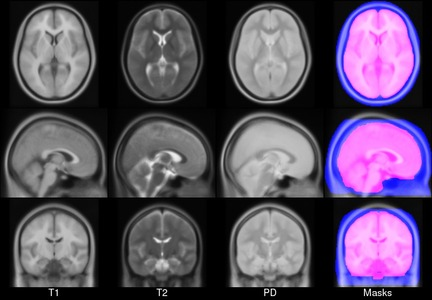
\includegraphics[scale=0.50]{mni_icbm152_lin.jpg}
    \centerline{Fonte: www.mcgill.ca}
    \label{fig:ICBMAtlas}
\end{figure}


\begin{figure}[h]
    \centering
    \caption{Modelo após a aplicação da máscara cerebral.}
    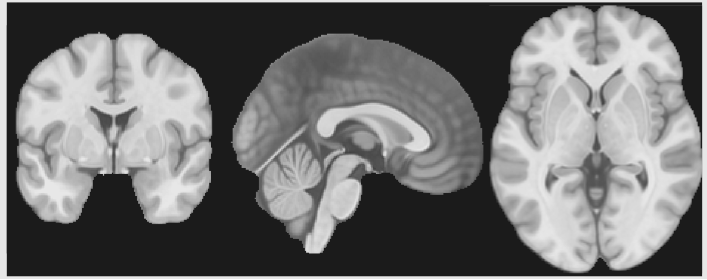
\includegraphics[scale=0.40]{depoisMask.png}
    \label{fig:depoisMask}
\end{figure}



%-------------------------------------------------------------


\begin{figure}[h]
    \centering
    \caption{Imagem original (\textit{ADNI{\_}023{\_}S{\_}0061{\_}MR{\_}MPR{\_}GradWarp})}
    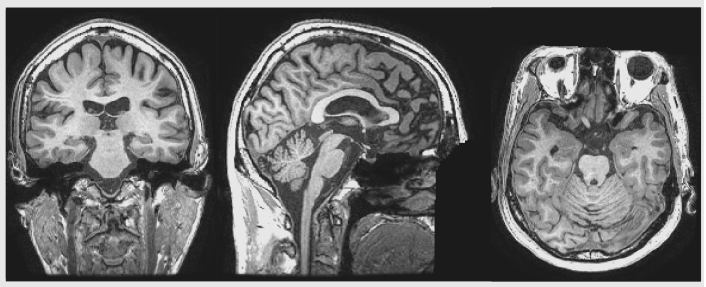
\includegraphics[scale=0.40]{MRIG3t1.png}
    \label{fig:MRIG3t1}
\end{figure}



\begin{figure}[h]
    \centering
    \caption{Imagem após Normalização}
    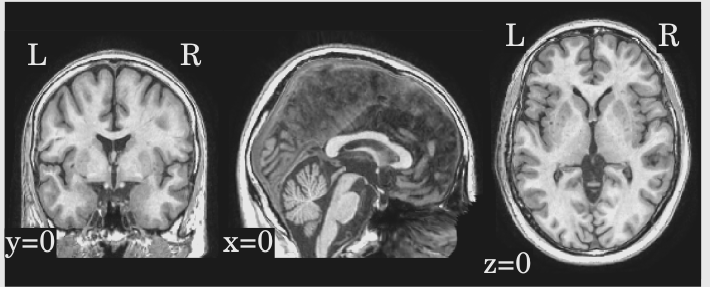
\includegraphics[scale=0.40]{MRIG3t1Normalization.png}
    \label{fig:MRIG3t1Normalization}
\end{figure}


\begin{figure}[h]
    \centering
    \caption{Imagem após a aplicação da máscara cerebral}
    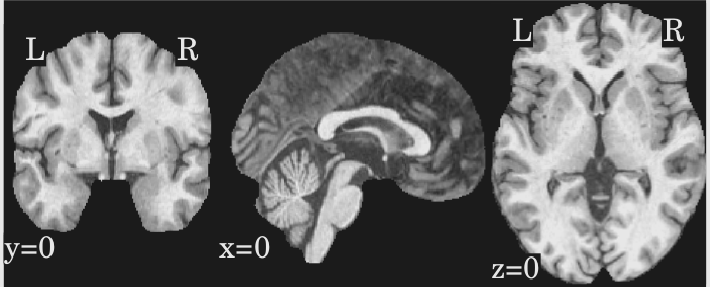
\includegraphics[scale=0.40]{MRIG3t1final.png}
    \label{fig:MRIG3t1final}
\end{figure}

Para ajudar no processo de segmentação também foi utilizado a ferramenta \textit{Medical Imaging NetCDF Toolkit} (MINC-TOOLKIT) também foi utilizado no processo de segmentação. O formato de arquivo MINC, bibliotecas e ferramentas fornecem uma estrutura para a manipulação de imagens médicas, independentemente da modalidade. O MINC 1.0 foi criado em 1993 para atender às necessidades da comunidade de pesquisa de imagens do cérebro. 
Os arquivos MINC 1.0 definem um sistema de coordenadas "voxel" 
e uma transformação em um "mundo" ou sistema de coordenadas estereotáxicas.
Os dados do "Voxel" podem incluir uma conversão de faixa opcional de um formato de
armazenamento inteiro para um formato de memória de ponto flutuante.

No processo de segmentação, foi necessário converter MRI no formato NIFTI (.nii) para extensão (.mnc), para usar MINC,
e então a máscara foi aplicada para remover o crânio do cérebro na 
imagem que, em nosso contexto de análise da doença de Alzheimer não é necessário. Após o processo de segmentação e normalização do cérebro, a imagem de saída tem a mesma dimensões como o atlas, ou seja, 193×229×193 px.
Com isso essa foi dimensão em pixel da imagem submetida no modelo de treinamento.


\section{Modelo proposto}

Nosso modelo de arquitetura utiliza uma estrutura de camadas  semelhante
a LeNet-5 \cite{lecun2015lenet}. A arquitetura LeNet-5 CNN é composta por 7 camadas. A composição das camadas consiste em 3 camadas convolucionais, 2 camadas de subamostragem e 2 camadas totalmente conectadas.
 A LeNet-5 é tida como uma rede \textit{shallow} (rasa) quando comparada com as arquiteturas  modernas, porém e importante ressaltar que mesmo arquitetura simples é possivel alcançar bons resultados \cite{lecun2015lenet}.

Na arquitetura proposta temos 7 camadas, assim como na arquitetura LeNet-5, porém algumas modificaçoes foram feitas. Basicamente o nosso modelo, foi composto das seguintes camadas
. Camada C1 (camada 1)  é composta por uma camada de convulução com um \textit{kernel} (3x3x3) e 62 neurônios de entrada. Na segunda camada C2 temos
32 neurônios, na proxima camada temos um \textit{MaxPooling} com um \textit{pool} de 3, pois foi mesmo que utilizamos na camada de convolução.
A operação de \textit{MaxPooling} retira o maior elemento de determinada matrix, (considerando o tamanho do \textit{pool} aplicado). Posteriormente, é feito um deslizamento considerado um parametro de \textit{stride} para aplicação de uma nova operação.


Também adicionamos \textit{batch
normalization}  para todas as camadas convolucionais e  as camadas totalmente conectadas. A normalização em lote ou  (\textit{batch
normalization})
 é uma técnica de normalização feita entre as camadas de uma rede neural  ao invés de se utilizar os dados brutos  diretamente. Isso é feito em peguenos lotes em vez de no conjunto de dados completo. Serve para agilizar o treinamento e 
utilizar taxas de aprendizado mais elevadas, facilitando o aprendizado \cite{ioffe2015batch}. A normalização em lote é uma técnica para padronizar as entradas de uma rede.
ela também ajuda acelera o treinamento, em alguns casos reduzindo as épocas à metade ou melhor, e fornece alguma regularização, reduzindo o erro de generalização. Todas as funções de ativação
ções foram unidades lineares retificadas (ReLU) , definidas como  $$ f (x) = max (0, x)  $$ , exceto para o
saída de classificação, que era uma função sigmoid. Finalmente, o número exato de camadas
ou profundidade variou de acordo com o padrão de rede adotado.


Naturalmente, na última camada temos uma camada com uma função de ativação sigmoid, pois no modelo proposto realizamos uma classficação binarias. A função sigmoid tem como característica produzir valores entre [0,1] como já mencionamos anteriormente, com isso conseguimos de foma binária (ativando vs não ativando) termos duas saidas proposta pelo modelo pessoas com AD ou pessoas normais AC . A função de ativação sigmoid e definida por  $$ \sigma '(x) = \ sigma (x) (1 - \ sigma (x)) $$


Na Figura  \ref{fig:cnnmodel}, temos  exemplo do modelo realizado com a abstração de algumas camadas ocultas, porém podemos ter uma ideia do modelo implementado. 
Podemos ver  que \textit{input} de entrada para rede é o "voxel". voxel é um elemento de volume ( pixel volumétrico ) que representa um valor no espaço tridimensional (expresso em unidades de  ${mm^3}$ ), correspondendo a um pixel para uma dada espessura de corte \cite{watkins2001structural}.

\begin{figure}[h]
    \centering
    \caption{Exemplo do Modelo CNN implementado}
    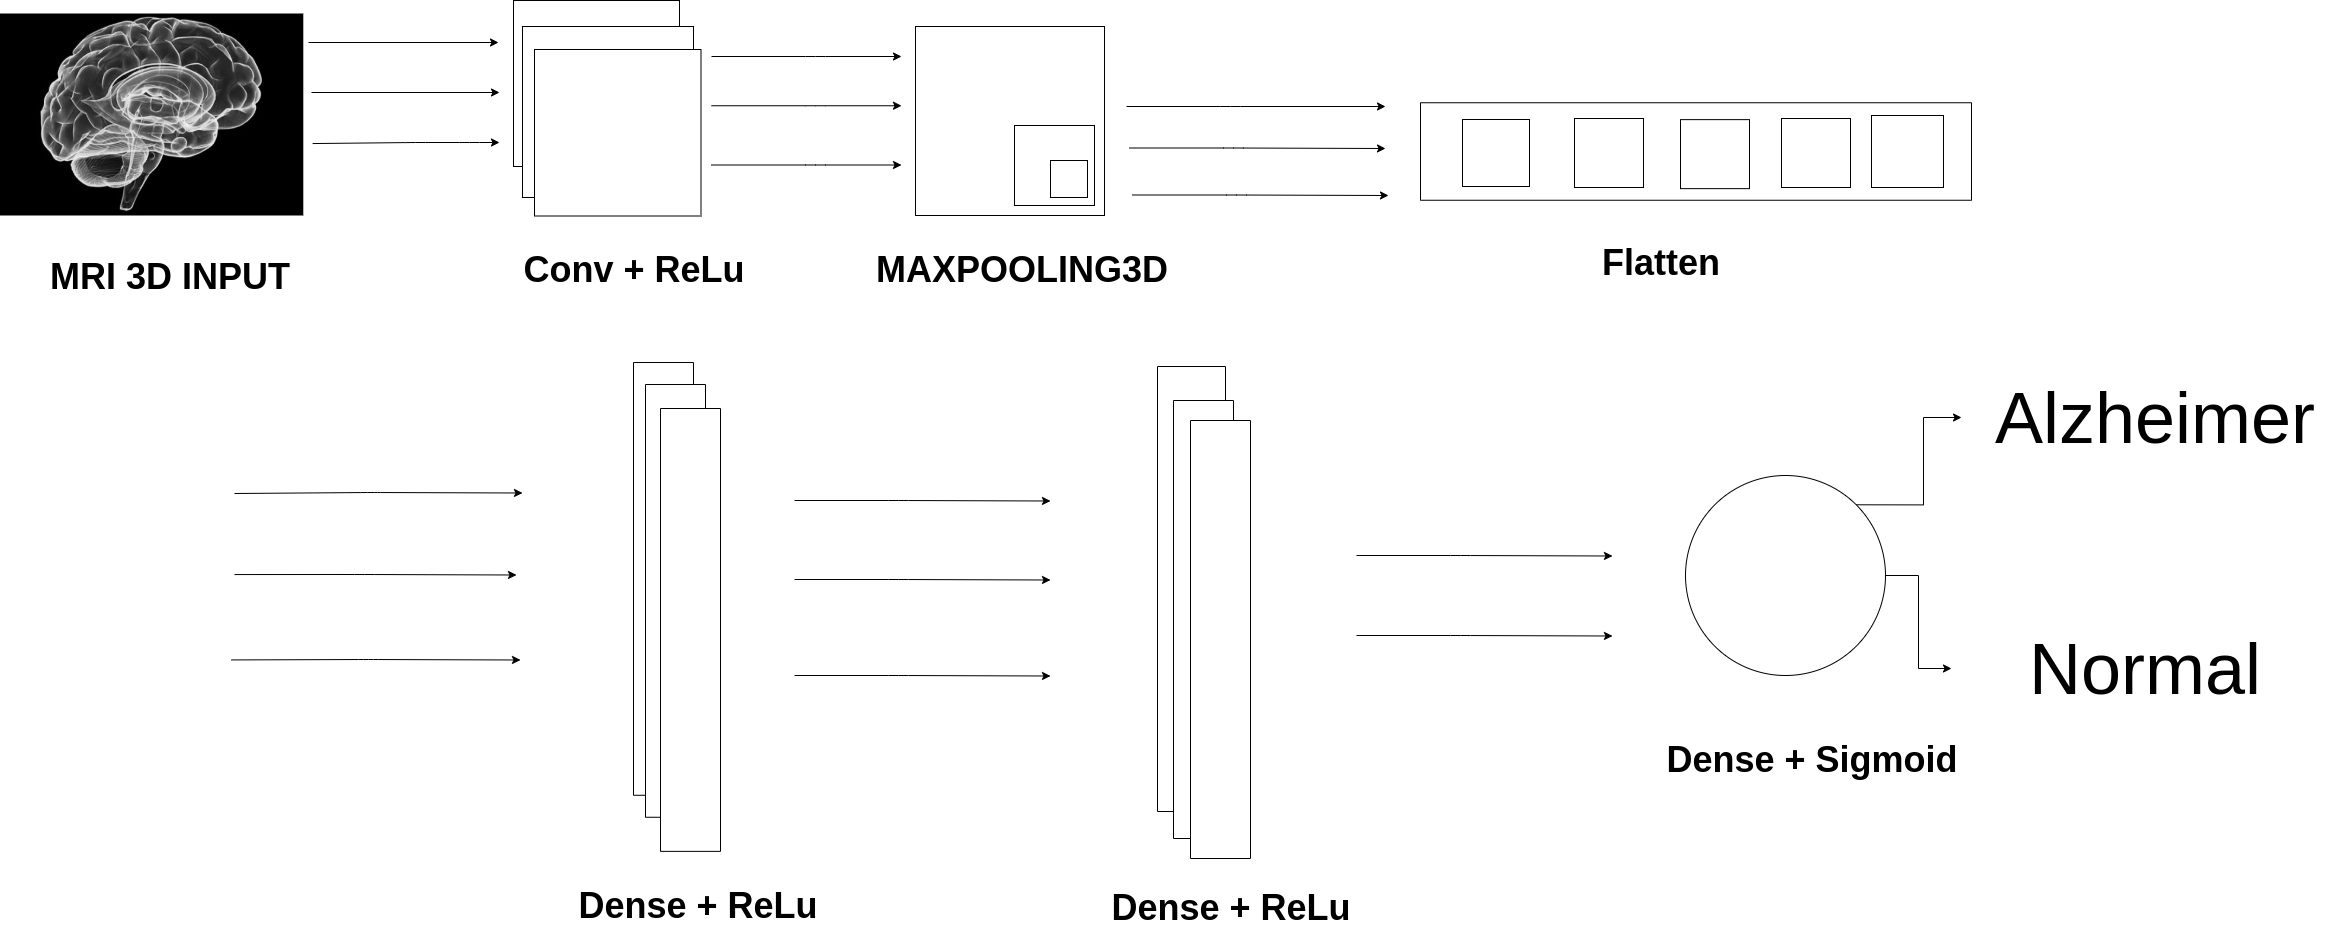
\includegraphics[scale=0.20]{cnn3d.png}
    \centerline{Fonte: autor}
    \label{fig:cnnmodel}
\end{figure}



Toda a arquitetura da rede e sua otimização foram implementadas usando Keras \footnote[1]{https://keras.io/}  e  Tensorflow \footnote[2]{https://www.tensorflow.org/}  (ou seja, a versão mais recente do repositório de código) TensorFlow  , que é uma biblioteca de código aberto criada para aprendizado de máquina, computação numérica e muitas outras tarefas. Foi desenvolvido pelo Google \cite{abadi2016tensorflow}. Também  foi utilizado  TensorFlow-GPU, que é uma extensão do TensorFlow para trabalhar com GPUs e poder utilizar  recursos do desenvolvimento com CUDA. 

A implementação do modelo desenvolvido foi utilizado liguagem de programação Python 3.8.5, CUDA 7.5 e CuDNN 5. Além disso, usamos algumas bibliotecas auxiliares como scikit-learn 0.24.0 , numpy 1.16.4 e matplotlib 3.3.4. 


Todos os experimentos foram conduzidos usando a seguinte configuração de hardware, 2 x (Intel Xeon E5-2650 v3 Haswell (Q3'14), 2,3 GHz) com 20 núcleos (10 por CPU), totalizando 100 núcleos e 200 threads, 128 GB DDR4 RAM, 2 x (NVIDIA TeslaK80, Kepler, 2 x 2496 Threads CUDA) de memória GPU.  Também foi utilizado um processador i7 com 4 cores físicos e 4 emulado, com memória RAM de 16GB e HD 2T.



\section{Experimentos e Resultados}

Esta Seção apresenta os resultados dos experimentos  realizados
nesse trabalho e tambem algumas metricas extraídas. Ao longo dos experimentos, diversas combinações de técnicas foram usadas para tratar os dados e parametrizar modelos, buscando o melhor desempenho na classificação. Para o nosso trabalho, utilizamos o método de \textit{Holdout}. O \textit{Holdout}  divide o seu conjunto de dados em 80-20 de maneira aleatória. Onde o 80 representa 80\% do seu conjunto de dados, que por sua vez será usado para treinar seu modelo e 20 os 20\% restantes para testar sua performance e validação \cite{kim2009estimating}.

Na Tabela \ref{results}  podemos verificar os resultados dos experimentos do método proposto. A tabela foi montada utilizando os melhores resultados capturados das interaçoes que foram rodados nos treinamentos realizados.
Tivemos alguns parametros que foram configurados de acordo com analise interaçoes de testagem do método. os  valores de \textit{epochs} aplicados foram respectivamente  $2,4,6$. Também foi atributido os valores de  \textit{batch\_size}  $4,6,8$. O \texit{dropout} utilizado em todos os treinamentos e testes foi de 0.2. O melhor resultado que obtivemos foi como mostra em destaque na tabela \ref{results}. Com configuração de parâmetros com os valores de  4  \textit{epochs} , \textit{batch\_size} 6 e \texit{dropout} 0.2. 



\begin{table}[h]
 \begin{center}
 \caption{Resultados por épocas }
\begin{tabular}{|l|l|l|l|l|}
\hline
Épocas & Acurácia & AUC    & Sensibilidade & Especificidade \\ \hline
2     & 0.8443    &  0.6427    &  0.5732                & 0.6341                \\ \hline
\textbf{4 }    & \textbf{0.8873}    & \textbf{0.7813} & \textbf{0.6652}        & \textbf{0.6554}         \\ \hline
6     & 0.79245   & 0.6221       &    0.6529           &     0.6257            \\ \hline

8    & 0.72245   & 0.5913       &    0.6167           &     0.59,42            \\ \hline
\end{tabular}
   \label{results}
\end{center}
\caption{Fonte: Acervo Pessoal}
\end{table}

As métricas analisadas foram  acurácia, sensibilidade, especificidade. A acurácia é a proximidade de um resultado com o seu valor de referência real. Dessa forma, quanto maior a acurácia, mais próximo da referência ou valor real é o resultado encontrado \cite{monico2009acuracia}
. Também usamos outras métricas para avaliar nosso modelo de classificação, \textit{Receiver Operating Characteristic Curve} (ROC).
A curva ROC mostra o quão bom o modelo criado pode distinguir entre duas coisas.
Uma curva ROC traça "Taxa de verdadeiro positivo versus taxa de falso positivo"  em diferentes limites de classificação.
Foi utilizado e também o calculo do valor da AUC métrica (área sob a curva ROC), onde obtivemos um valor AUC de 0,7813. Na Figura  \ref{fig:rocCurve} podemos ver a curva ROC do modelo implementado, essa, curava teve os parametros configurados com \texit{ddropout}.
Acreditamos que os resultados podem melhorar,
embora para validar esta teoria sejam necessários mais experimentos. O codigo fonte do modelo implementado esta disponivel no Gihub \footnote{
https://gist.github.com/augustoberwaldt/50b46be801281c4b3b0d04a8a8b0817f}.



\begin{figure}[h]
    \centering
    \caption{Curva ROC do Modelo Prosposto CNN 3D}
    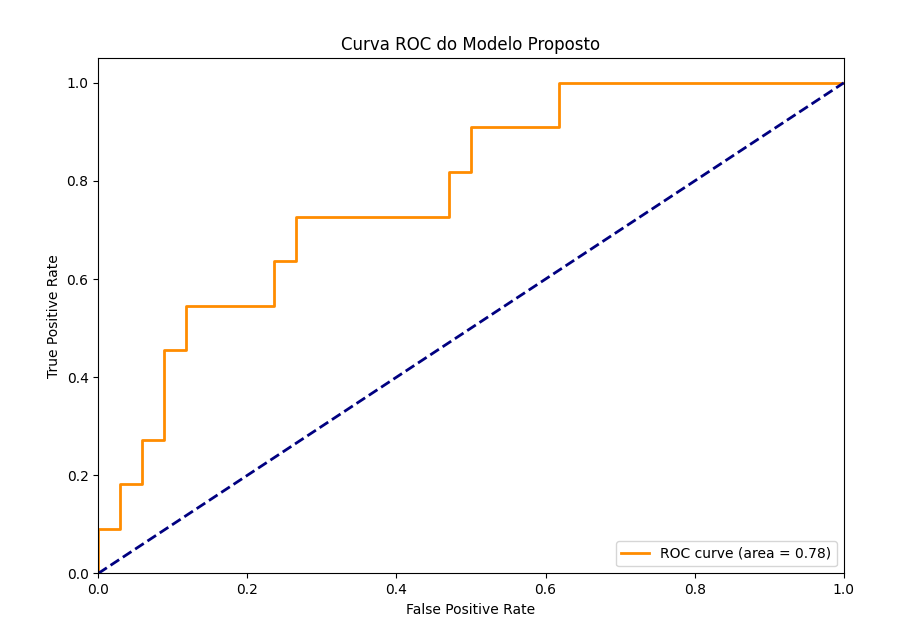
\includegraphics[scale=0.40]{ROCCurvemodelopro.png}
    \centerline{Fonte: Acervo Pessoal}
    \label{fig:rocCurve}
\end{figure}


De forma a comparar o metodo porposto, comparamos com metodo do trabalho de \cite{rieke2018visualizing}, onde os autores realizam  imagens de MRI, utilizando  \texit{deep learning}, mais precisamente o modelo  utiliza conceito de redes \texit{autoencoder} para realizar a classificação, para mais detalhes ver capítulo 3. Se comparamos nosso resultado com o resultado dos autores podemos verificar que obtivemos, valores proximos de AUC, e valor superior de acurácia. Assim como nosso modelo proposto aqui, os autores \cite{rieke2018visualizing}, também utilizaram base de dados ADNI e eles também utilizaram como parâmetro de entrada voxel para o modelo de treinamento implementado. Diferença que podemos observar nos trabalhos é parte de pré-processameto das imagens onde tivemos duas abordagens diferentes. A arquitetura dos modelos também foi distinta onde \cite{rieke2018visualizing}  os autores utilizaram uma arquitetura de modelo baseada no modelo de \cite{khvostikov20183d}.

\chapter{Conclusão}

Este trabalho propôs o desenvolvimento de um modelo de \textit{deep learning}, que pode classificar imagens de MRI,
utilizando pre-processamento de imagem, para depois realizar classificação das imagens. Para esste fim, foi proposto modelo de uma rede CNN com dados
volumétricos, onde os dados sumetidos a rede passaram por um processo de
normalização e adequação dos dados. Também foi necessário  remover partes da imagem que não eram  necessárias para o objetivo do modelo. Foi realizado  extração do crânio da MRI, para poder trabalhar somente com cérebro e o volume da massa cinzenta. Analisando os resultados, podemos perceber que o método proposto tem potencial para futuras aplicações na área de processamento digital de imagens utilizando Inteligência Artificial.

Uma das aplicações possíveis deste trabalho, é facilitar a triagem de pacientes, além de possibilitar um histórico de imagens e análises para acompanhamento  do quadro do paciente, para possíveis estudos sobre o tipos de demência  e também sobre doenças de Alzheimer.


O método elaborado aplica-se com melhor desempenho em cenários de classificação
binária, com utilização de aprendizagem supervisionada. Observando os cenários executados, percebemos os melhores resultados em cenários onde os pacientes não estão em
uma faixa intermediária da progressão da doença (distúrbios cognitivos leves). A aplicação da segmentação nas imagens mostrou um aprimoramento considerável nos resultados, removendo atributos desnecessários e realçando os relevantes. A grande vantagem utilizar técnica que utilizamos no pre-procesamento das MRI é que ferramenta e de fácil uso, onde falicita extração \texit{features} das imagens, e também que possui um comunidade bastante ativa, utilizando ANTS.

Os resultados alcançados, com o uso de metricas da validação foram 
comparado com   RIEKE et al, onde metodo proposto obteve valor mais significativo de acurácia. Podemos comparar também nossos resultados com
o desafio proposto por CADDementia (https://caddementia.grand-challenge.org/). onde é proposto desafio de criação de classificador para análise de imagens MRI, de pessoas com AD, MCI e NC. 


Devo comentar que as dificuldades também compõem a conclusão do método e testes desenvolvidos. O grande problema em trabalhar com
modelos 3D de dados é capacidade  \texit{hardware} limitada para implementação do modelo, o que acaba atrapalhando muito na busca de melhores resultados. Como base de dados utilizada tinha bastante objetos/MRI, tratar  um volume de dados grande acaba sendo custoso.
Cada imagem tinha aproximandamente 14.16 MB  no seu formato original, onde foi disponibilizado pelo ADNI. Alguns testes foram  aplicados utilizando 
\textit{downsampling}, porém os resultados não foram satisfatórios, por isso optamos por não utilizar \textit{downsampling}. 
Uma consideração importante de resaltar é que não utilizamos técnica de regularização \textit{data augmetation}, pois um dos motivos é que o \textit{dataset} 
tinha quantidade 
significativa de imagens e também  por  que segundo Faceli (2011)  não é considerado uma boa pratica aplicar essa técnica em imagens clinicas/médicas,
pois segundo Faceli (2011) pode-se adicionar algum ruído na imagem ou ate mesmo ocorrer um \textit{underfitting}.



\chapter{Trabalhos Futuros}


Como trabalhos futuros pretende-se estender a variação de parâmetros para avaliação, como a quantidade de camadas convolucionais da rede, a fim de maximizar os resultados observando as métricas definidas para análise. Além disso,pretende-se realizar um estudo de uma abordagem que utilize imagens segmentadas contendo pontos de regiões de interesse utilizando redes convolucionais. Outra abordagem pretendida é investigar aplicação de técnicas de balanceamento de dados em imagens para entrada de redes convolucionais.


Outros interesses de experiências futuras, seria trabalhar com classificação multiclasse, também ter  diferentes fontes de dados para obter uma maior variabilidade do modelo. Usar também outros tipos de imagens, como tomografia computadorizada ou até mesmo PET-SCAN (Tomografia de Emissões Posi-tron). Outro possivel estudo seria  testar outros modelos de CNN com maiores camadas, e selecionando
algumas areas do cérebro com auxilio de um profissional de Neurociência. Outros objetivos que podem ser aprimorados  para  pesquisas futuras com intuito  de termos melhor resultados e desempenho:

\begin{itemize}
 \item Devem ser pesquisadas técnicas de emsemble, visto que redes neurais consolidadas
na literatura estão sendo utilizadas em conjunto para gerar melhores resultados.

 \item Utilizar  processamento paralelo e distribuído para o pre-processamento das imagens, fazendo essa parte ter processmento mais
 rapido e que facilite normalização e segmentação das imagens.

\item Utilizar a técnica de cross-validation.

\end{itemize}





% carrega o arquivo com as bibliografias e põe o capítulo com as referências neste lugar
\bibliography{bibliografia}

% a partir daqui, todo capítulo novo é apêndice
% \appendix

% \chapter{Anexos e Apêndices}
% Destinam-se à inclusão de informações complementares ao trabalho, mas que não são essenciais à sua compreensão. Os Apêndices devem apresentar material desenvolvido pelo próprio autor, formatado de acordo com as normas. Já os Anexos destinam-se à inclusão de material como cópias de artigos, manuais, etc., que não necessariamente precisam estar em conformidade com o modelo, e que não foram desenvolvidos pelo autor do trabalho.

%importa dicasLatexABNT.tex para o Apêndice 
% \chapter{Dicas de Latex e Normas ABNT}
Esta capítulo apresenta as coisas básicas que precisamos saber para fazer um TCC com Latex utilizando este modelo.

\section{O Básico do Latex}
Novo parágrafo pode ser feito por meio do comando par. \par
Outra forma é deixando uma linha em branco entre dois parágrafos.

Tudo o que está a direita de um \% é um comentário.
% Isto é um comentário
Para inserirmos o símbolo de porcento de forma proposital, precisamos colocar a barra invertida antes: 90\%.

Os caracteres \& \$ \# \% \_ \{ \} \^{} \~{} $\backslash$ são todos especiais e precisam ser escritos como comandos (com uma barra antes).
% tem um web app para ajudar a encontrar outros símbolos neste endereço: http://detexify.kirelabs.org/classify.html

Aspas são digitadas com duas crases no início e duas aspas simples no final: ``Texto entre aspas''; ou com o comando say: \say{Texto entre aspas}.

Estilos de fontes: \emph{ênfase} (sempre destaca o texto, mesmo que este já esteja em negrito/itálico), \textbf{negrito}, \textit{itálico}, \textrm{romano}, \textsf{sans serif}, \texttt{máquina de escrever}, \textsc{caixa alta}.

Capítulos, seções e subseções são inseridas com:
\begin{verbatim}
\chapter{Um Capítulo} -> 1 Um Capítulo
\section{Uma Seção} -> 1.1 Uma Seção
\subsection{Uma Subseção} -> 1.1.1 Uma Subseção
\subsubsection{Uma Subsubseção} -> 1.1.1.1 Uma Subsubseção
\chapter*{Um Capítulo} -> Um Capítulo sem numeração
\end{verbatim}
Não se deve utilizar mais do que 4 níveis.

Ambientes são utilizados para definir uma região do texto que haverá tratamento especial:

\begin{verbatim}
O ambiente verbatim significa "ao pé da letra". 
Ex.: & $ # % _ { } ^ ~ $
\end{verbatim}

\begin{center}
O ambiente center escreve centralizado.
\end{center}

\begin{quote}
O ambiente quote é útil para fazer citações.
\end{quote}

Esta é a forma como se descreve itens:
\begin{description}
\item[Item 1] Isto significa uma coisa.
\item[Item 2] Este significa outra coisa.
\end{description}

Esta é a forma como se cita itens:
\begin{itemize}
\item Item 1;
\item Item 2.
\end{itemize}

E esta é a forma como se enumera itens:
\begin{enumerate}
	\item Qual a alternativa correta?
		\begin{enumerate}
			\item esta.
			\item ou esta.
		\end{enumerate}
\end{enumerate}

Fórmulas matemáticas são colocadas dentro de um ambiente matemático. Tudo neste ambiente é considerado elemento numérico e possui uma formatação diferente. Os comandos aceitos também podem mudar.

Equações matemáticas em destaque são inseridas da seguinte maneira:

% tem um web app para ajudar a fazer equações neste endereço: http://mathurl.com/
% ou aqui: http://webdemo.visionobjects.com/#/demo/equation
$$
x=\frac{-b\pm\sqrt{b^2-4ac}}{2a}.
$$

ou 

\begin{equation}
\begin{array}{rcl}
x_2 - x_1 &\geq& b_1 r_1\\
x_2 - x_1 &\geq& b_2 r_2\\
x_2 - x_1 &\geq& b_n r_m\\
b_1 + b_2 + ... + b_n &=& 1
\end{array}
\end{equation}

enquanto equações inline são feitas desta forma: $r_i (1\leq i \leq m)$.

\section{Convenções}
Escreva o título e os capítulos, seções, subseções, etc. sempre com a primeira letra de cada palavra importante em Maiúsculo e o restante em minúsculo. O Latex se encarregará de deixar tudo MAIÚSCULO onde for necessário.

Nenhuma seção deve ficar sem texto.

Utilize siglas para não ter de repetir muitas vezes o mesmo texto. Neste caso, na primeira ocorrência coloque o significado antes e a sigla entre parênteses (aproveitando também para adiciona-la à lista de siglas). Nas demais ocorrências, apenas coloque a sigla. 
Ex.: ...com a execução do algoritmo de \textit{Threshold Accepting} (TA) sobre um circuito. A versão do algoritmo de TA utilizada...

Palavras em \textit{English} ou outra língua estrangeira devem estar em itálico. Utilize \textbf{negrito} quando for necessário destacar alguma coisa.

\section{Figuras e Tabelas}

Todas as figuras e tabelas devem estar referenciadas no texto e com a descrição acima delas. Não são permitidos outros nomes tais como: quadro, imagem, etc. Comece a descrição com letra maiúscula e faça o restante em minúscula (exceto siglas), terminando com um ponto final.

Se buscada em alguma obra publicada, a citação deve sempre aparecer. Pode ser colocada entre parênteses, como no exemplo da Figura \ref{fig:dsp2}, ou preferencialmente abaixo após a palavra "Fonte: ", como no exemplo da Tabela \ref{tab:comp1} e da Figura \ref{fig:dsp}. Observando que na LISTA DE FIGURAS/TABELAS a fonte/citação não deve aparecer.

É possível colocar as figuras de lado e também redimensiona-las através dos parâmetros do Latex, como nos exemplos das Figuras \ref{fig:dsp} e \ref{fig:dsp2}. Dê preferência por imagens vetoriais ou em PDF, para não perder qualidade. Procure deixar os textos das figuras com o mesmo tamanho das letras no restante do documento.

\begin{figure} % [h] -> utilize este parâmetro para forçar nesta posição
    \center{
    \caption{Segundo a ABNT, a descrição deve ficar acima da figura.}
    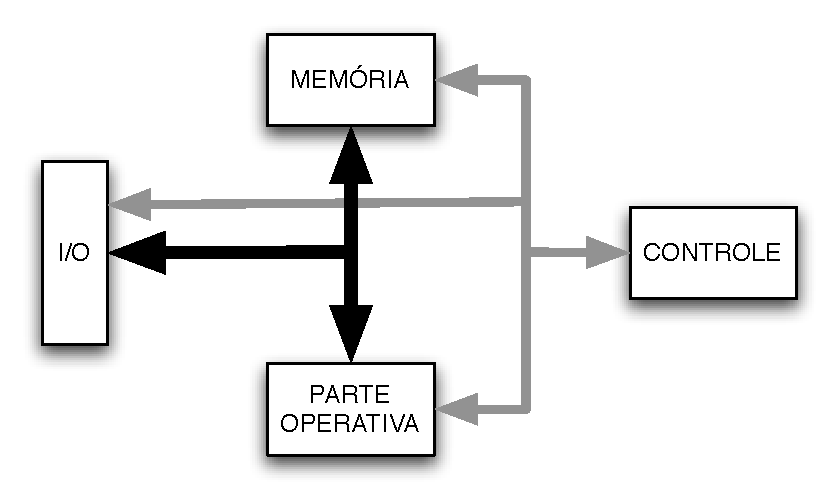
\includegraphics[width=20em]{figuras/dsp}\\
    Fonte: Elaborado pelo autor.}
    \label{fig:dsp}
\end{figure}

\begin{sidewaysfigure}
    % entre colchetes a descrição que vai para a lista de figuras, sem citação (parâmetro opcional mas que é necessário devido a norma da ABNT)
    \caption[Descrição com citação]{Descrição com citação \cite{artigo}.}
    \centerline{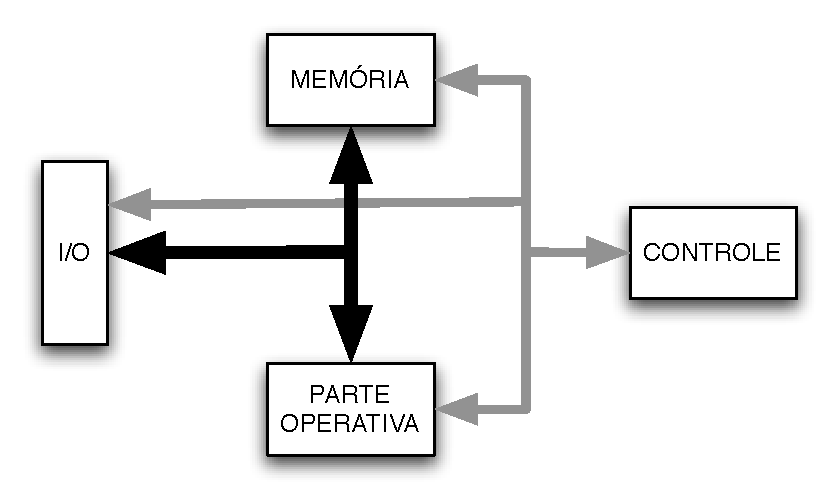
\includegraphics[width=40em]{figuras/dsp}}
    \label{fig:dsp2}
\end{sidewaysfigure}

As tabelas devem ser ``abertas'' dos lados (sem as linhas laterais), como no exemplo da Tabela \ref{tab:comp1}, isto torna a imagem mais limpa e clara.

% tem um web app para ajudar a fazer tabelas no Latex neste endereço: http://truben.no/latex/table/
\begin{table}
    \centering
    \scalefont{0.93} %necessário eventualmente para reduzir o tamanho da tabela
    \caption{Comparação entre X e Y.}
    \begin{tabular}{c|c|c|c|c|c} \hline
        \multirow{2}{*}{\textbf{Célula}} & \multirow{2}{*}{\# \bf{Trans.}} & \multicolumn{3}{|c|}{\bf{Largura} ($\mu m$)} & \bf{Tempo Exec. (s)}\\ \cline{3-6} 
         &  & Std. Cell & ASTRAN & \% & ASTRAN \\ \hline \hline
        AND2X4& 6 & 1 & 1,2 & 20 & 10 \\ \hline
        FAD1X4& 28 & 3,6 & 4 & 12 & 750\\ \hline
        FAD1X9& 28 & 4,2 & 4,2 & 0 & 1800\\ \hline
        HAD1X9& 14 & 2,4 & 2,4 & 0 & 30\\ \hline
        HAD1X18& 18 & 2,8 & 2,8 & 0 & 205\\ \hline
        INVX0 & 2 & 0,6 & 0,6 & 0 & 1\\ \hline
        TOTAL& - & 28 & 29 & 3,6 &-\\ \hline
    \end{tabular}
    {\\ Fonte: \cite{artigo}}
    \label{tab:comp1}
\end{table}

\section{Citações}
Há duas formas de se fazer uma citação: a citação indireta ou livre e a citação direta ou textual. Todas as citações devem trazer a identificação de sua autoria.

No Latex, inserimos citações utilizando o formato bibtex. Para tanto, precisamos cadastrar os dados da citação no arquivo .bib e em seguida citarmos no .tex com o comando cite. Colocar preferencialmente em ordem cronológica, com o mais recente por último \cite{livro, artigo, tese, capitulo, paper, site, apresentacao}.

\subsection{Citação Indireta}
Aquela citação na qual expressamos o pensamento de outra pessoa com nossas próprias palavras. Por esta razão seu uso é mais recomendado, pois demostra interpretação do autor sobre a obra citada. Ex.:

Segundo o trabalho de Silva e Santos \citeyearpar{artigo}, o céu é azul porque...

O céu é azul porque... \cite{artigo}.

\subsection{Citação Direta}
São aquelas em que se transcreve exatamente as palavras do autor citado. As citações diretas ou textuais podem ser breves ou longas. São consideradas breves aquelas cuja extensão não ultrapassa três linhas e devem vir entre aspas. As citações com mais de três linhas são chamadas de longas (sem aspas) e devem receber um destaque especial com recuo.  Ex.:

Segundo Silva, ``Quando a luz passa através de um prisma, seu espectro é dividido em sete cores monocromáticas'' \citeyearpar{artigo}.

\begin{quote}
Quando a luz passa através de um prisma, seu espectro é dividido em sete cores monocromáticas, eis que surge um arco-íris de cores. A atmosfera faz o mesmo papel do prisma, atuando onde os raios solares colidem com as moléculas de ar, água e poeira e são responsáveis pela dispersão do comprimento de onda azul da luz. \cite{artigo}
\end{quote}

Havendo supressão de trechos dentro do texto citado, faz-se a indicação com reticências entre colchetes [...]. De forma similar, para interpelação, acréscimo ou comentário durante a citação, deve-se fazê-lo também entre colchetes. No início ou no fim da citação, as reticências são usadas apenas quando o trecho citado não é uma sentença completa.Ex.:

``Também chamado de corpo do trabalho, [o desenvolvimento] tem por finalidade expor [...] a explicitação do assunto a ser abordado...'' \cite{artigo}.

\section{Notas de Rodapé}
As notas de rodapé\footnote{Nota sobre a palavra rodapé} são usadas nos documentos impressos para explicar ou fazer comentários detalhados.


\end{document}
